In this section mockups of the user interfaces are presented; an app for the final Users and a site for the \acp{CPO}\\
\subsection{User}
The user is whoever wants to use the service to book and manage charges trough the app. The mockups only represent the idea of the app, the actual design could differ based on the OS on which the app is implemented (different operating systems could provide different gestures/features to enhance the users experience).\\
It is assumed that the user has already installed the correct version of the app compatible with his/hers operating system.\\
The user can close every popup by clicking outside of it (in the grey area).
\subsubsection{Login}
\begin{figure}[H]
    \centering
    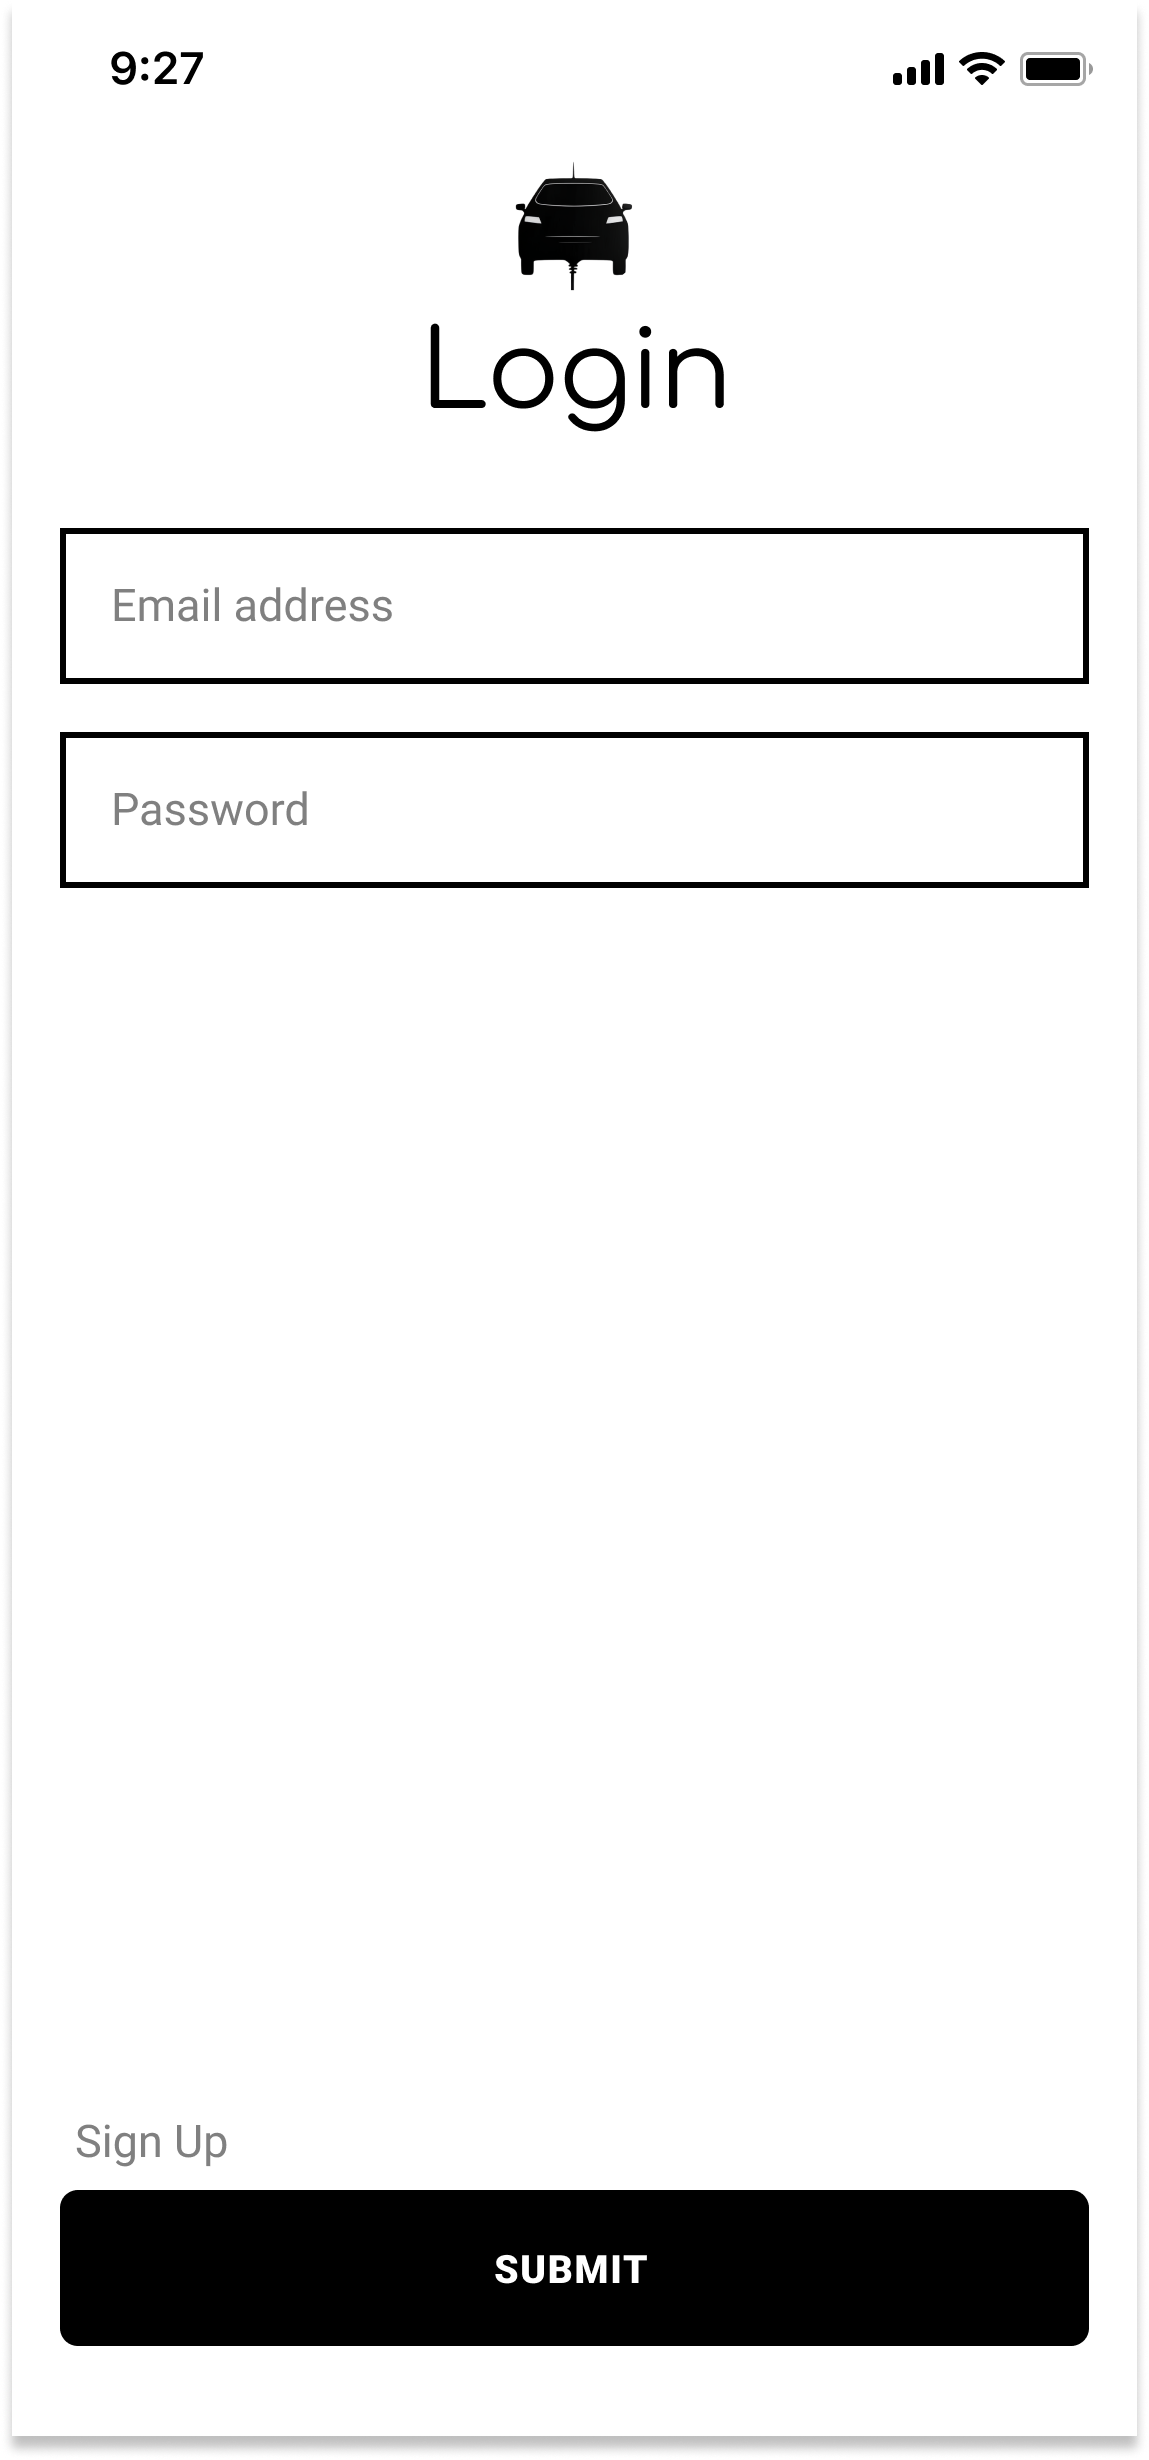
\includegraphics[keepaspectratio, height=15cm]{AppInterface/Login.png}
    \caption{User Logs in}
    \label{fig:Login}
\end{figure}
The first time the user opens the app he/her is prompted to log in by inserting email and password in the corresponding field and pressing the submit button. If the information provided are correct the \hyperref[fig:Search]{search station page} is displayed; otherwise the \hyperref[fig:FailedLogin]{failed login page} is shown.\\
The user can press the Sign Up button to open the \hyperref[fig:Register]{register page}.
\begin{figure}[H]
    \centering
    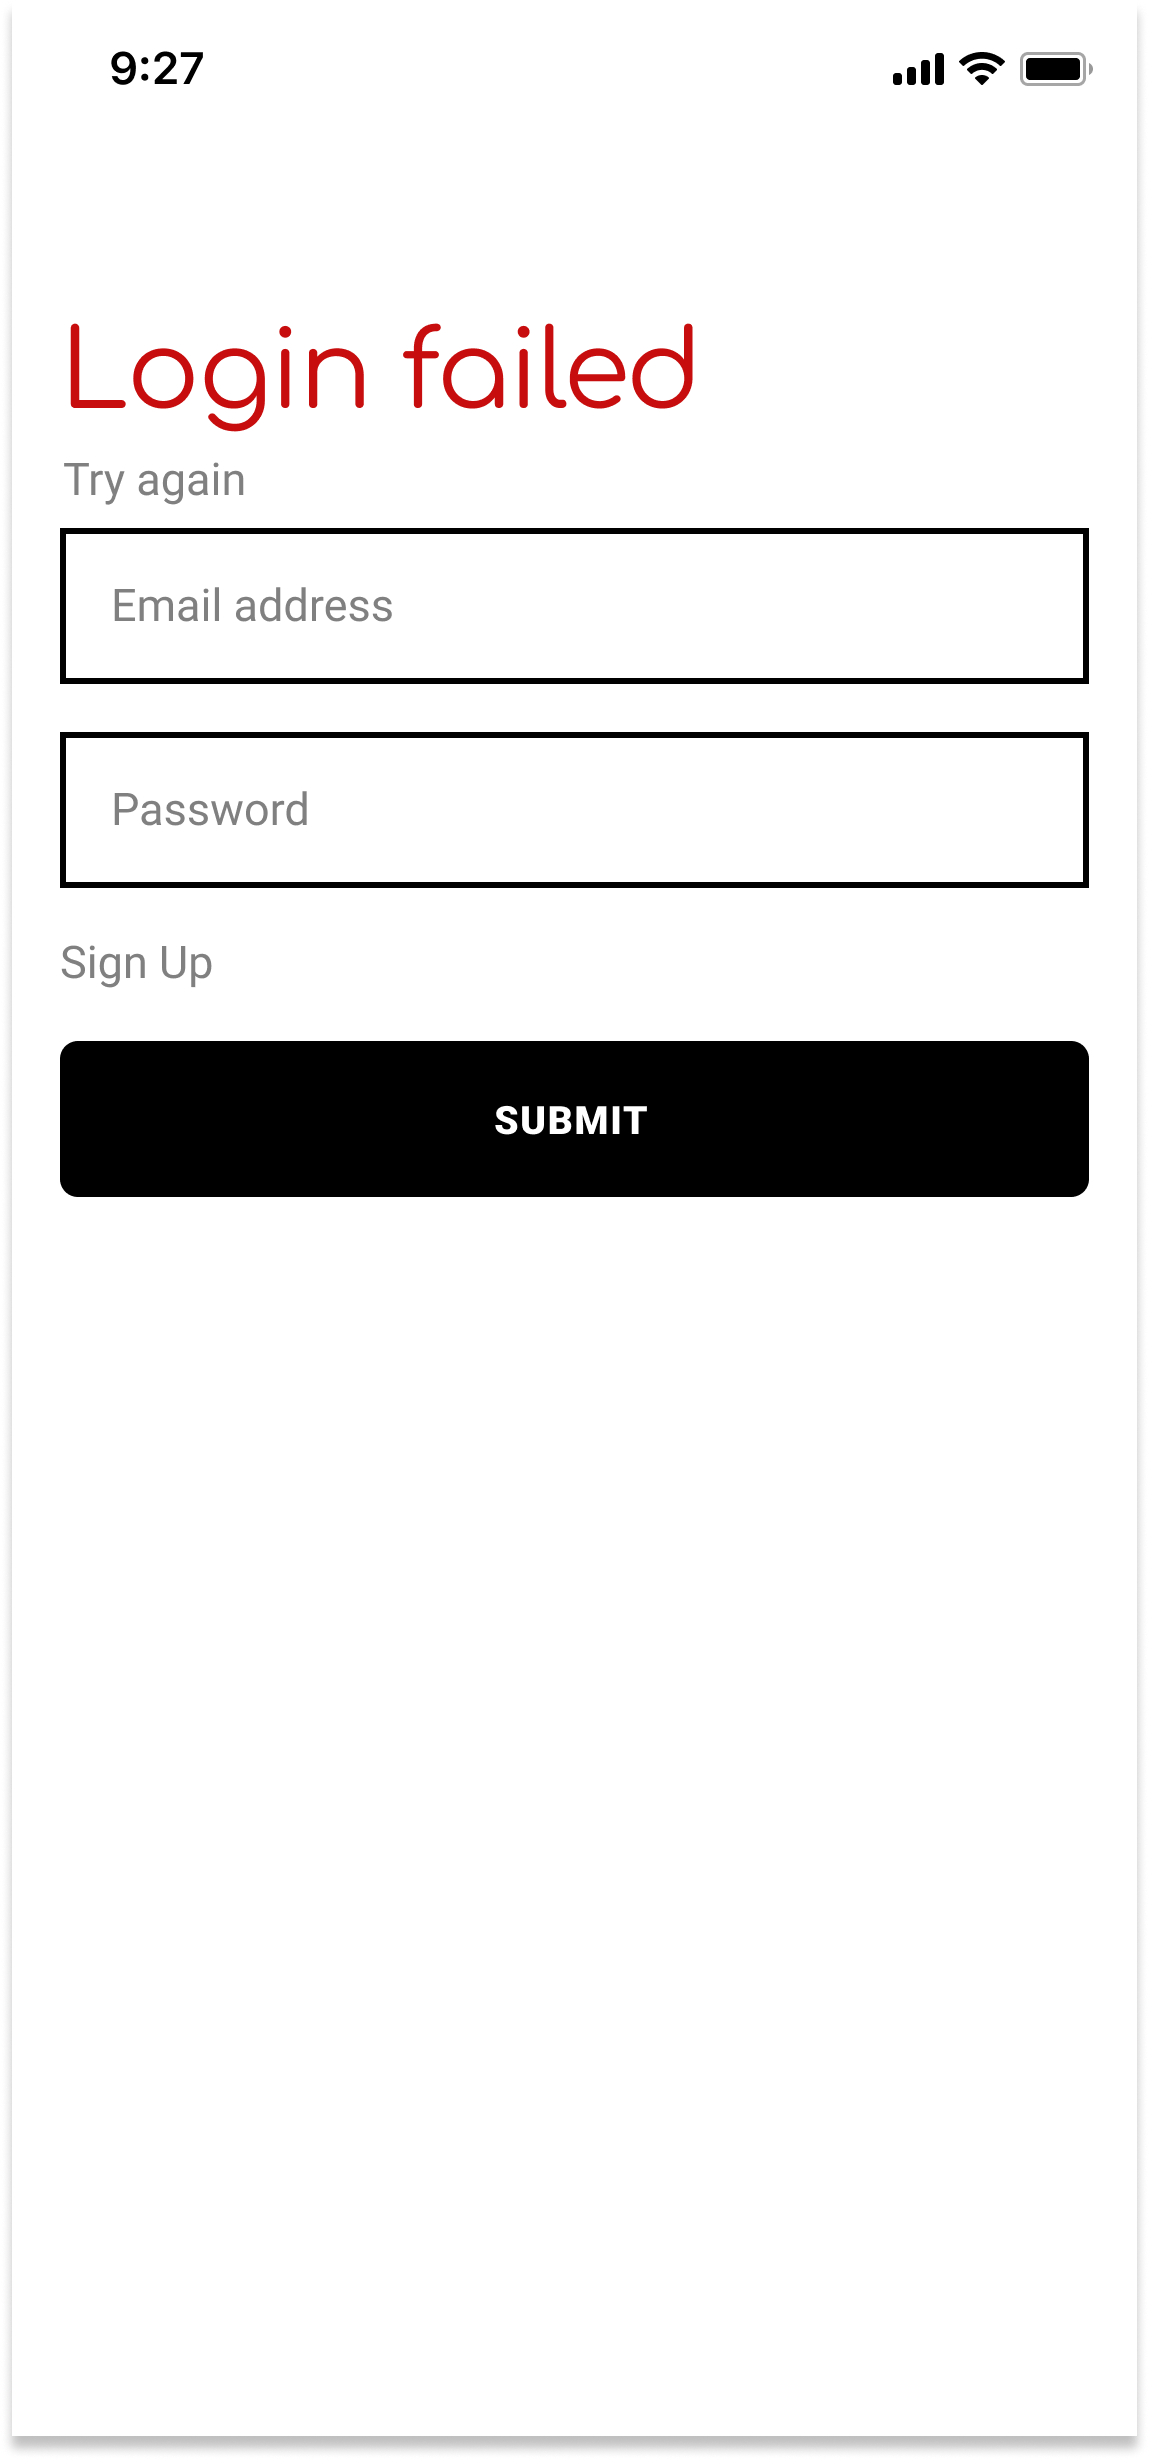
\includegraphics[keepaspectratio, height=15cm]{AppInterface/Failed Login.png}
    \caption{Wrong Credential}
    \label{fig:FailedLogin}
\end{figure}
If the user has inserted the wrong email or password he/she can retry it in this page, otherwise the user can press the Sign Up button to open the \hyperref[fig:Register]{register page}.


\subsubsection{Register}
\begin{figure}[H]
    \centering
    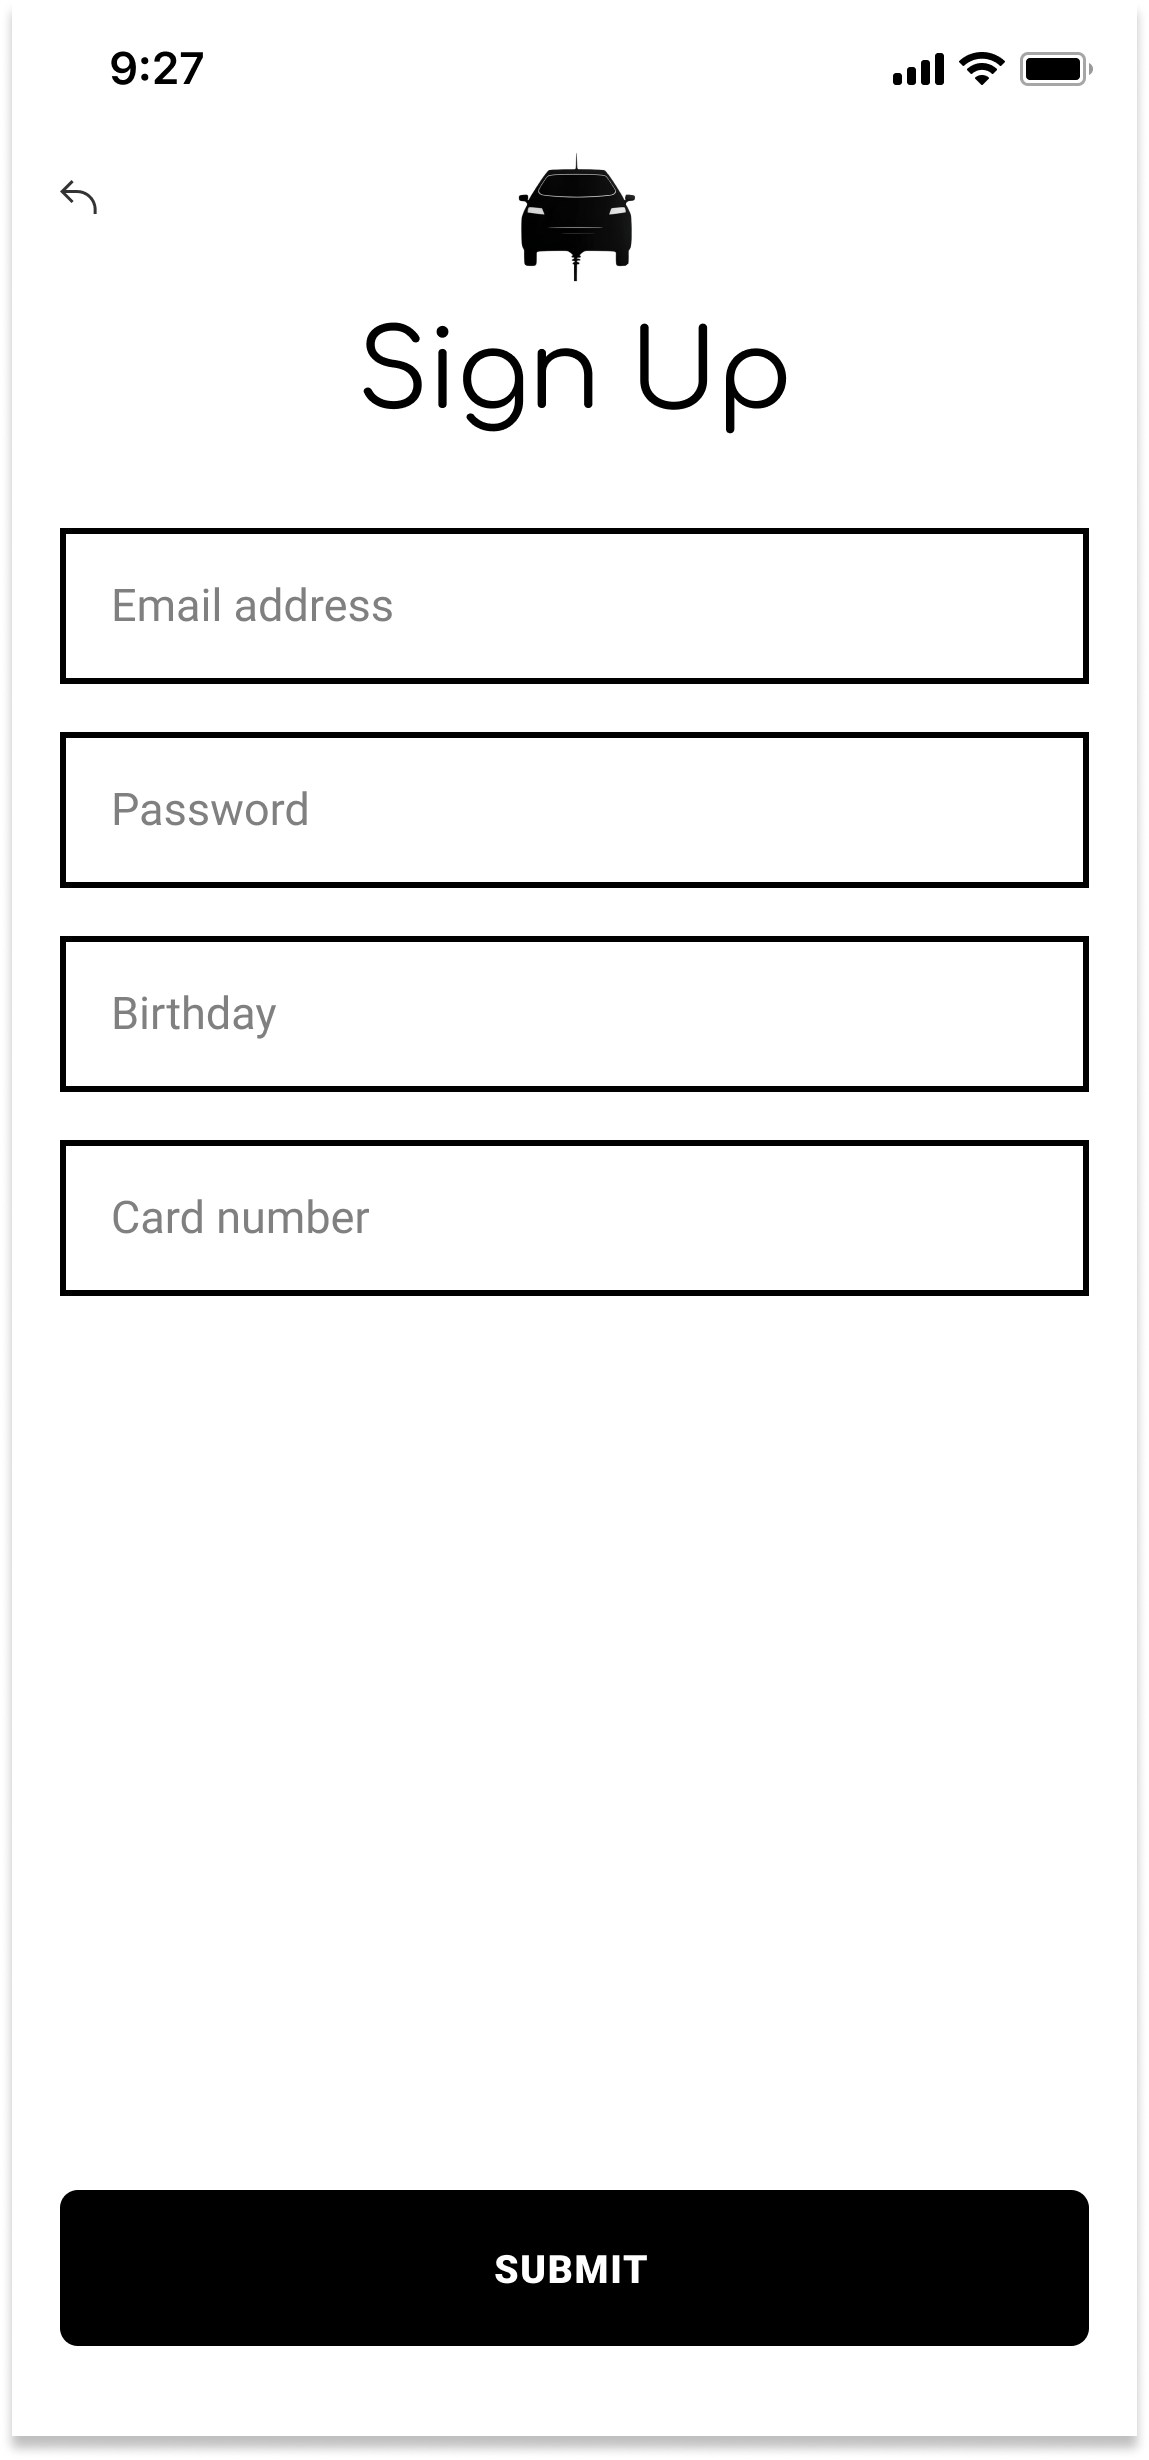
\includegraphics[keepaspectratio, height=15cm]{AppInterface/Register.png}
    \caption{User Register}
    \label{fig:Register}
\end{figure}
If the user has not already registered himself/herself he/her can do it here by inserting the right data in the corresponding fields and pressing the submit button.\\
After the Sign up procedure is completed the \hyperref[fig:Login]{login page} is displayed and the user has to log in.
If the user wants to return to the \hyperref[fig:Login]{login page} he can do so by pressing the backward arrow in the top left corner.\\
\subsubsection{Search a Station}
At any screen shown in this section the user can press the car logo at the top to load the \hyperref[fig:myCharges]{manage charges page}
\begin{figure}[H]
    \centering
    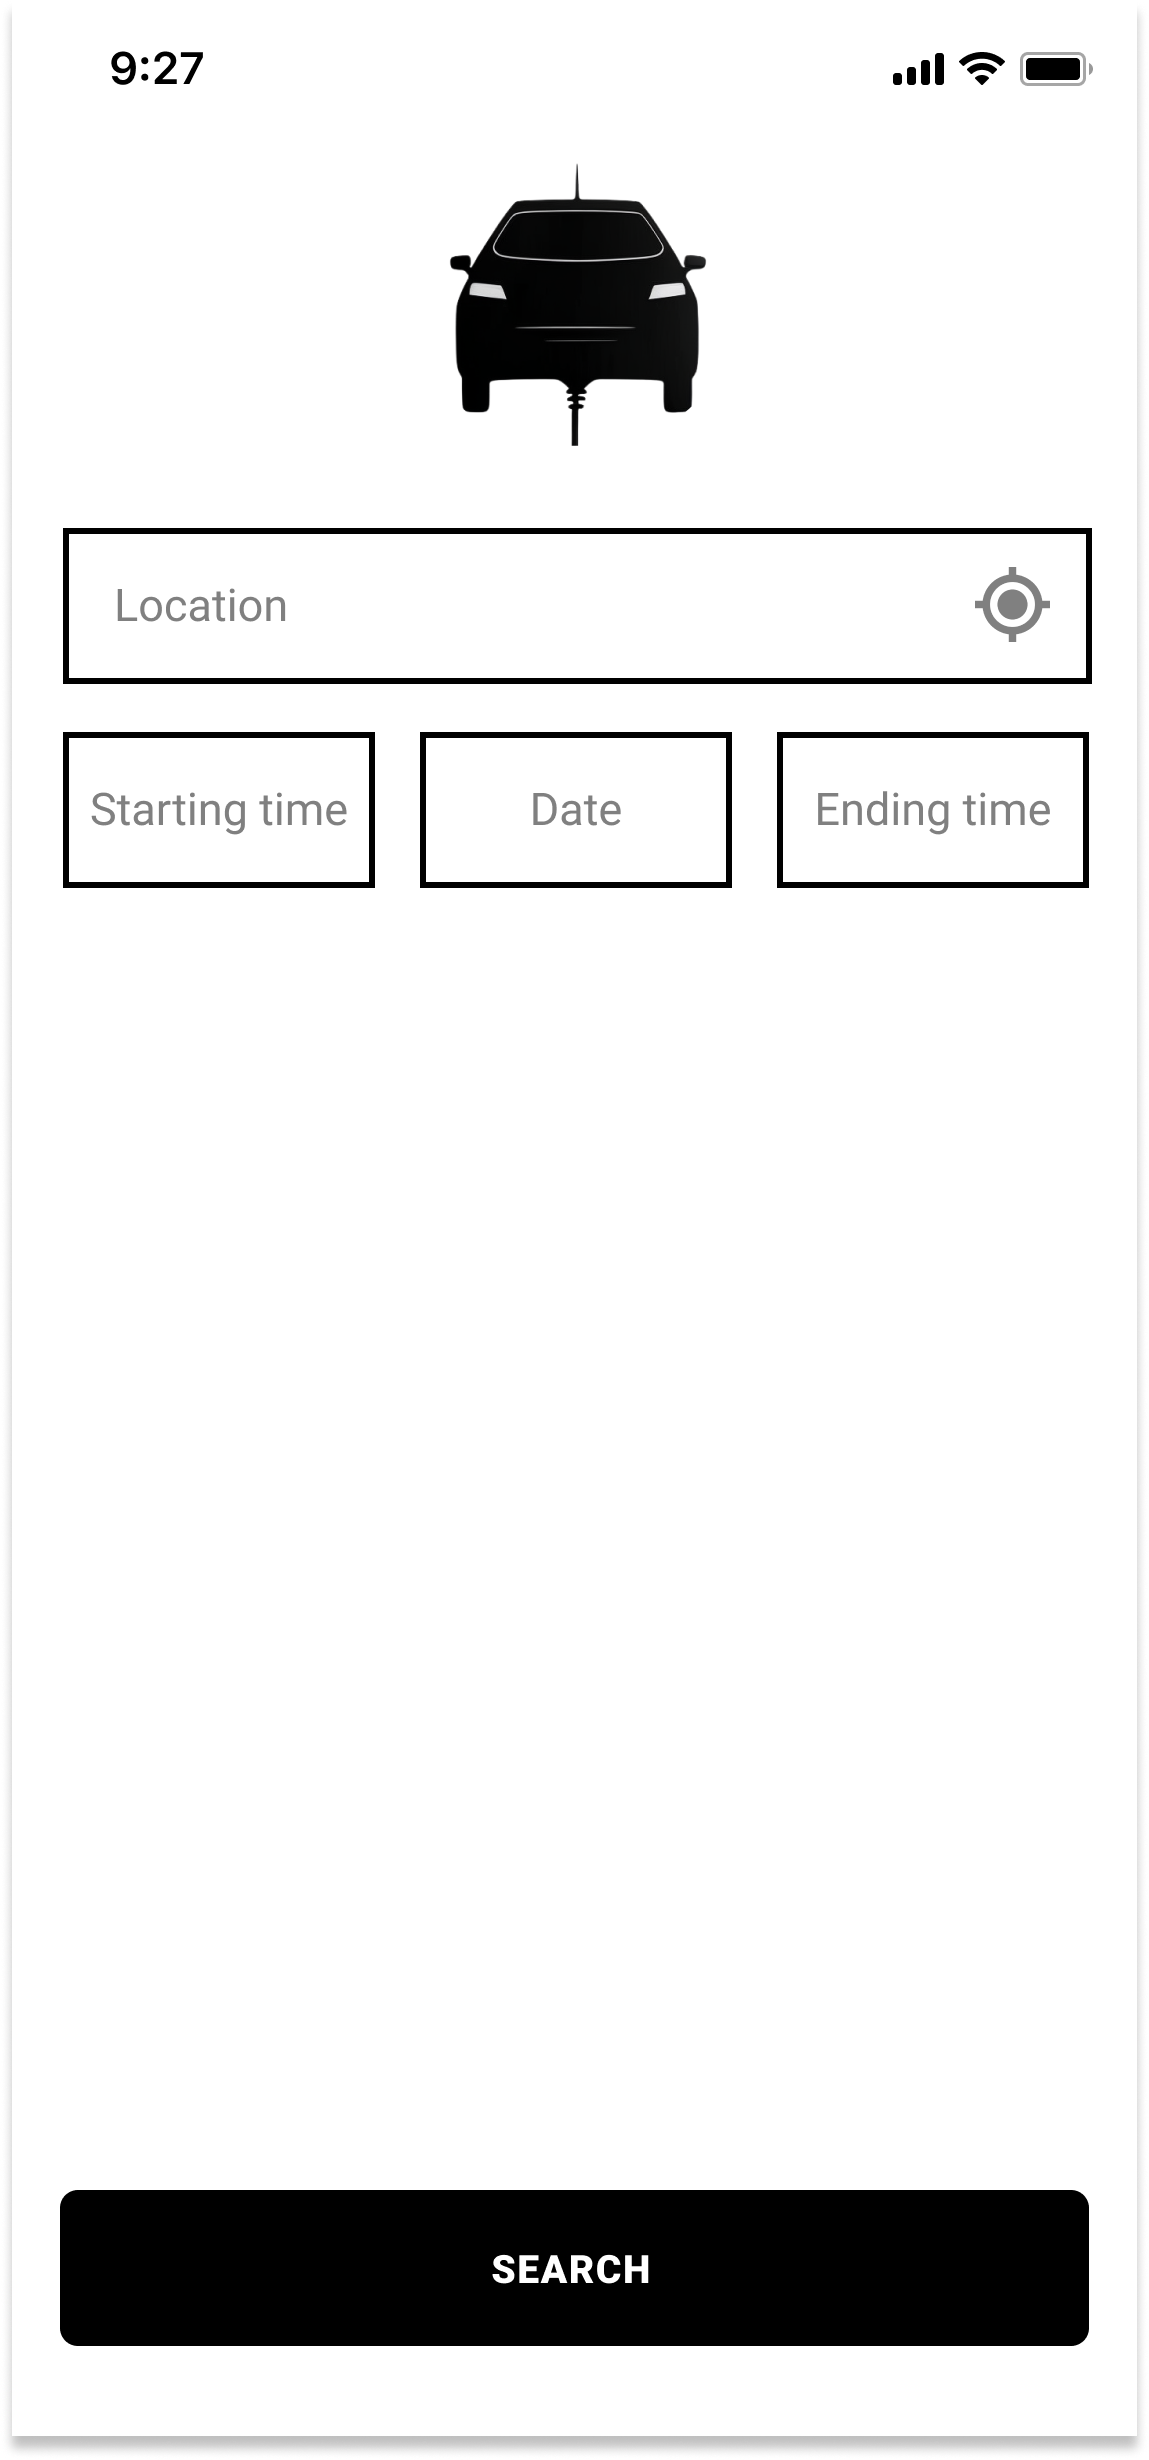
\includegraphics[keepaspectratio, height=15cm]{AppInterface/Station Search.png}
    \caption{User Search for Stations}
    \label{fig:Search}
\end{figure}
In this section the user can search for stations by inserting the location, the starting and ending time for the charge. By pressing the location icon the user can automatically use his current location.
Once the data are inserted the user can press Search to advance to the \hyperref[fig:Results]{results page}.
\begin{figure}[H]
    \centering
    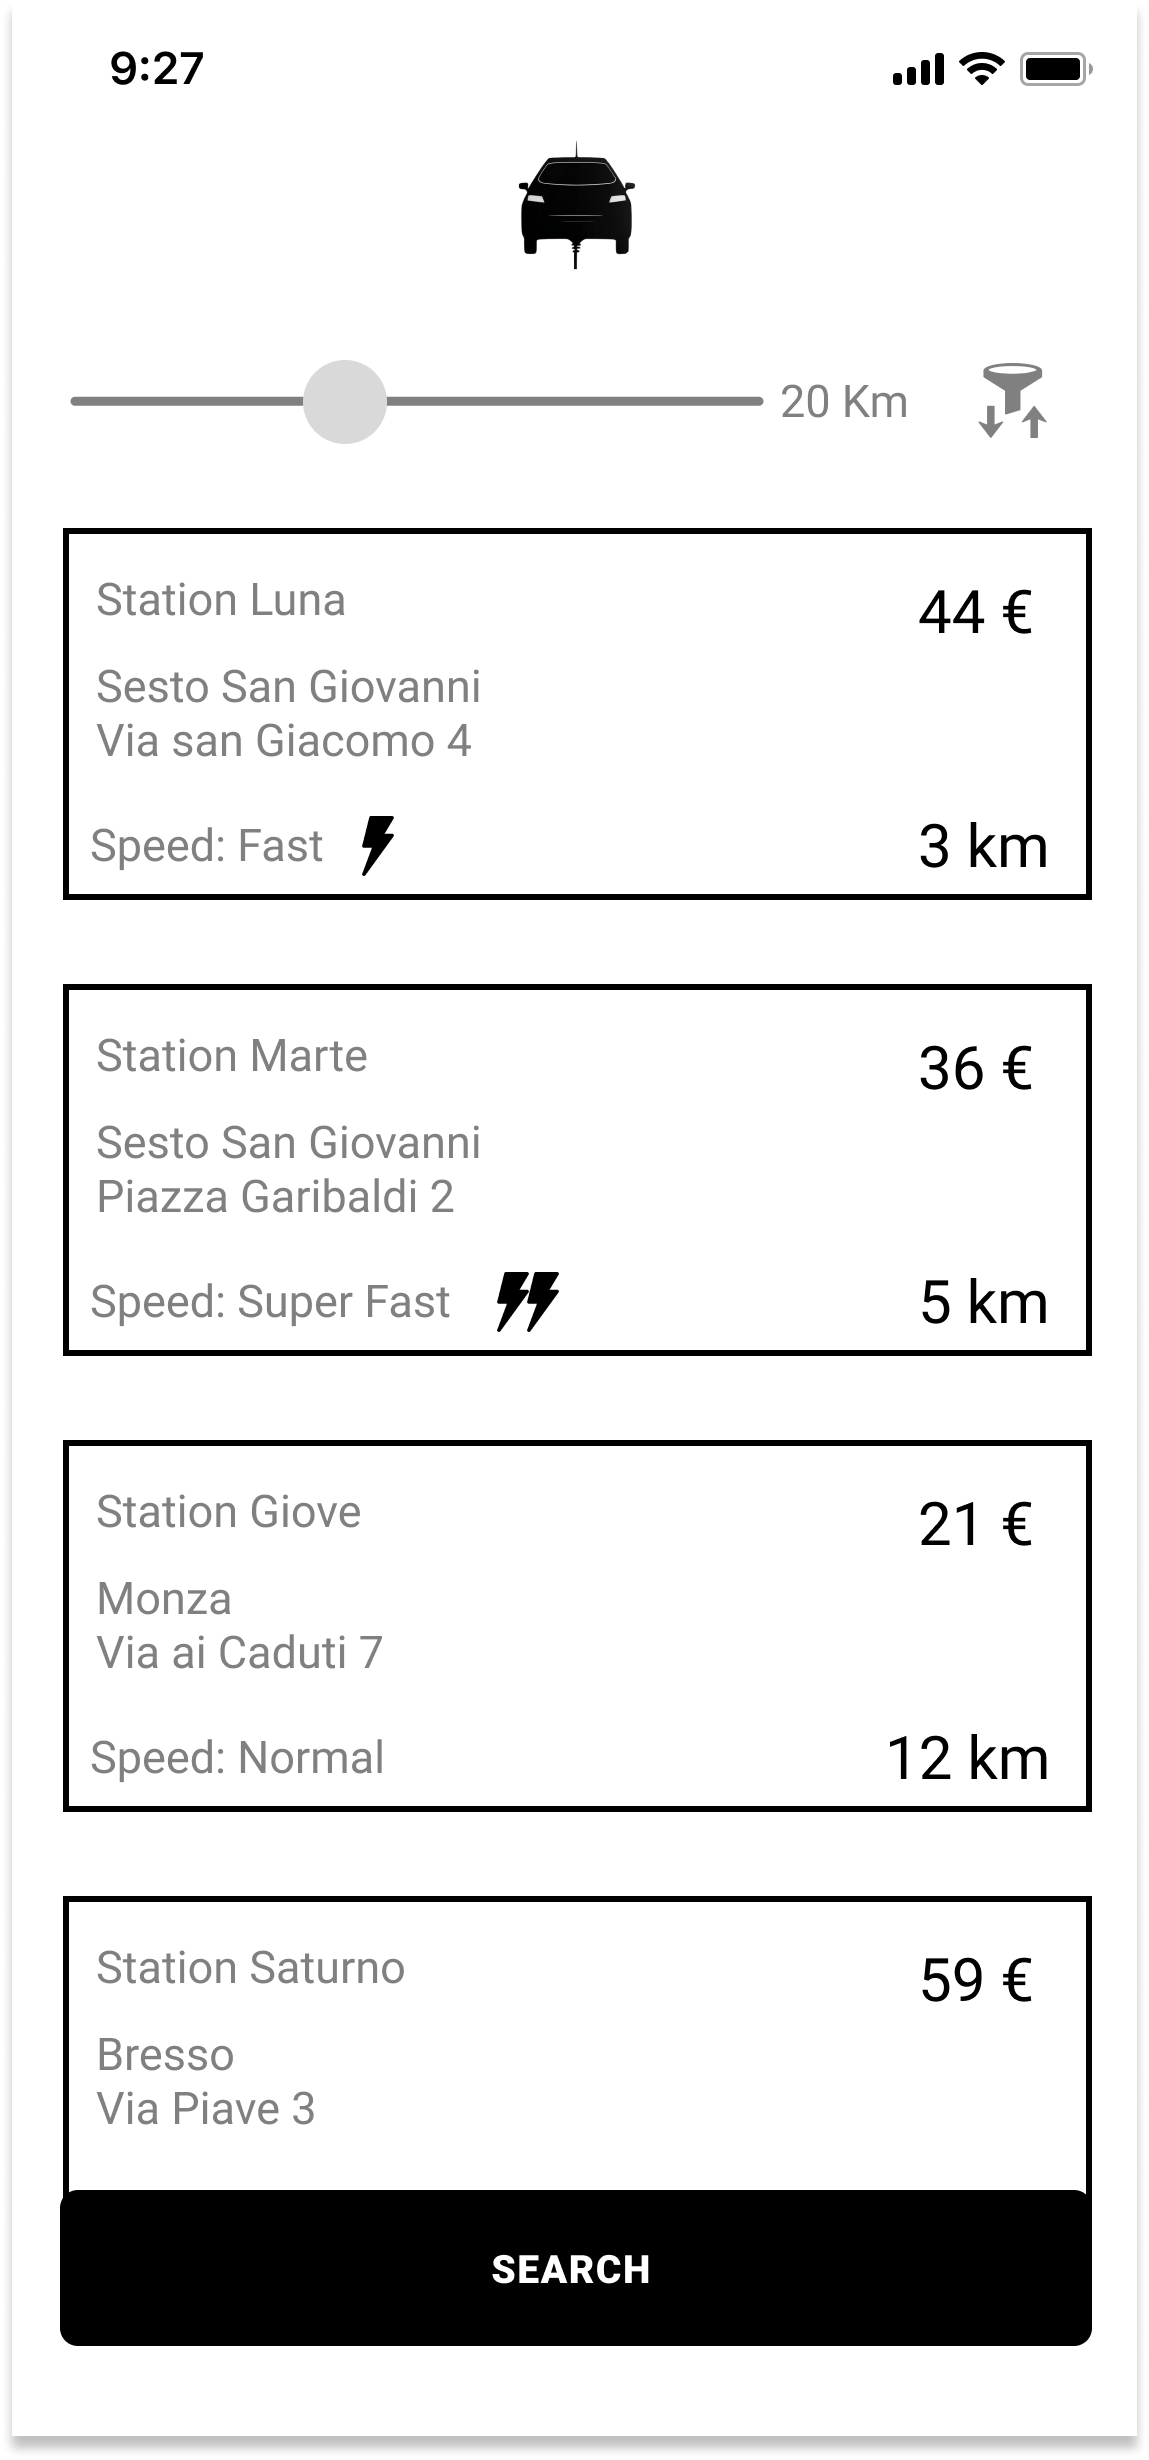
\includegraphics[keepaspectratio, height=15cm]{AppInterface/Results.png}
    \caption{Search results}
    \label{fig:Results}
\end{figure}
Here the user is shown the results of the search, using the slider on top the user can change the radius of search from the given position, at the right of the slide the selected distance is shown; at the most right the filter icon is displayed, if pressed the \hyperref[fig:Filters]{filter popup} is showed.\\
A list of station with their details is displayed (station name, location, speed, distance from selected location and price of the charge), clicking on a station opens that \hyperref[fig:StationDetails]{station details page}. Pressing the Search button allow the user to make another search trough the \hyperref[fig:Search]{search station page}.
\begin{figure}[H]
    \centering
    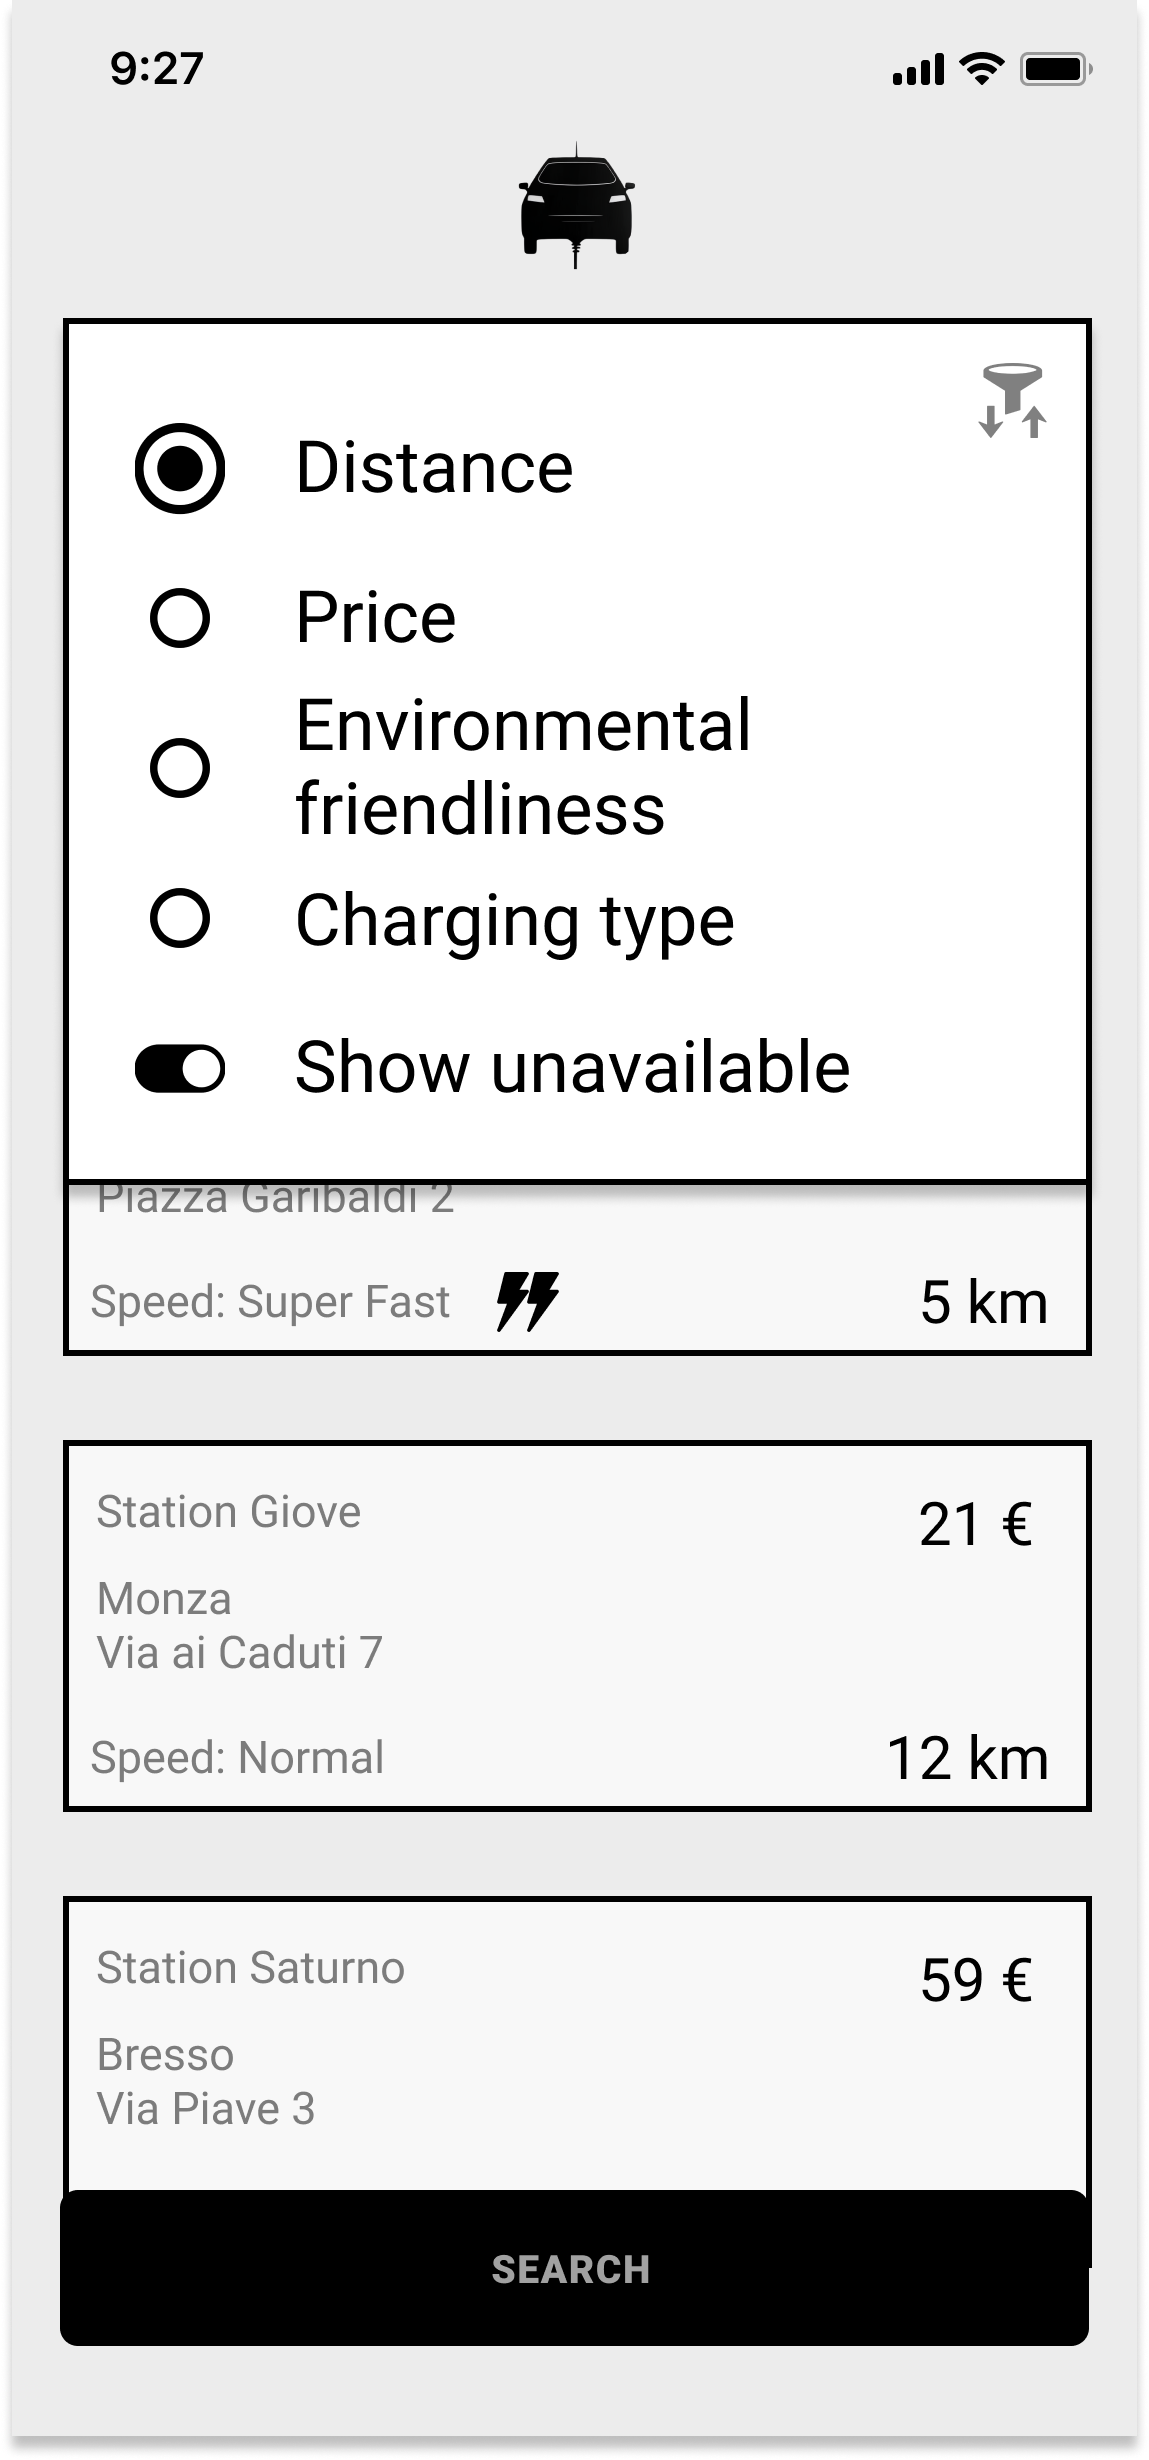
\includegraphics[keepaspectratio, height=15cm]{AppInterface/Filter Menu.png}
    \caption{User Filters the Results}
    \label{fig:Filters}
\end{figure}
In this popup the user can select whether to sort the results by distance, price, environmental friendliness or charging type via a radio button, and to show or to not show unavailable station trough the toggle.

\subsubsection{Book a Station}
\begin{figure}[H]
    \centering
    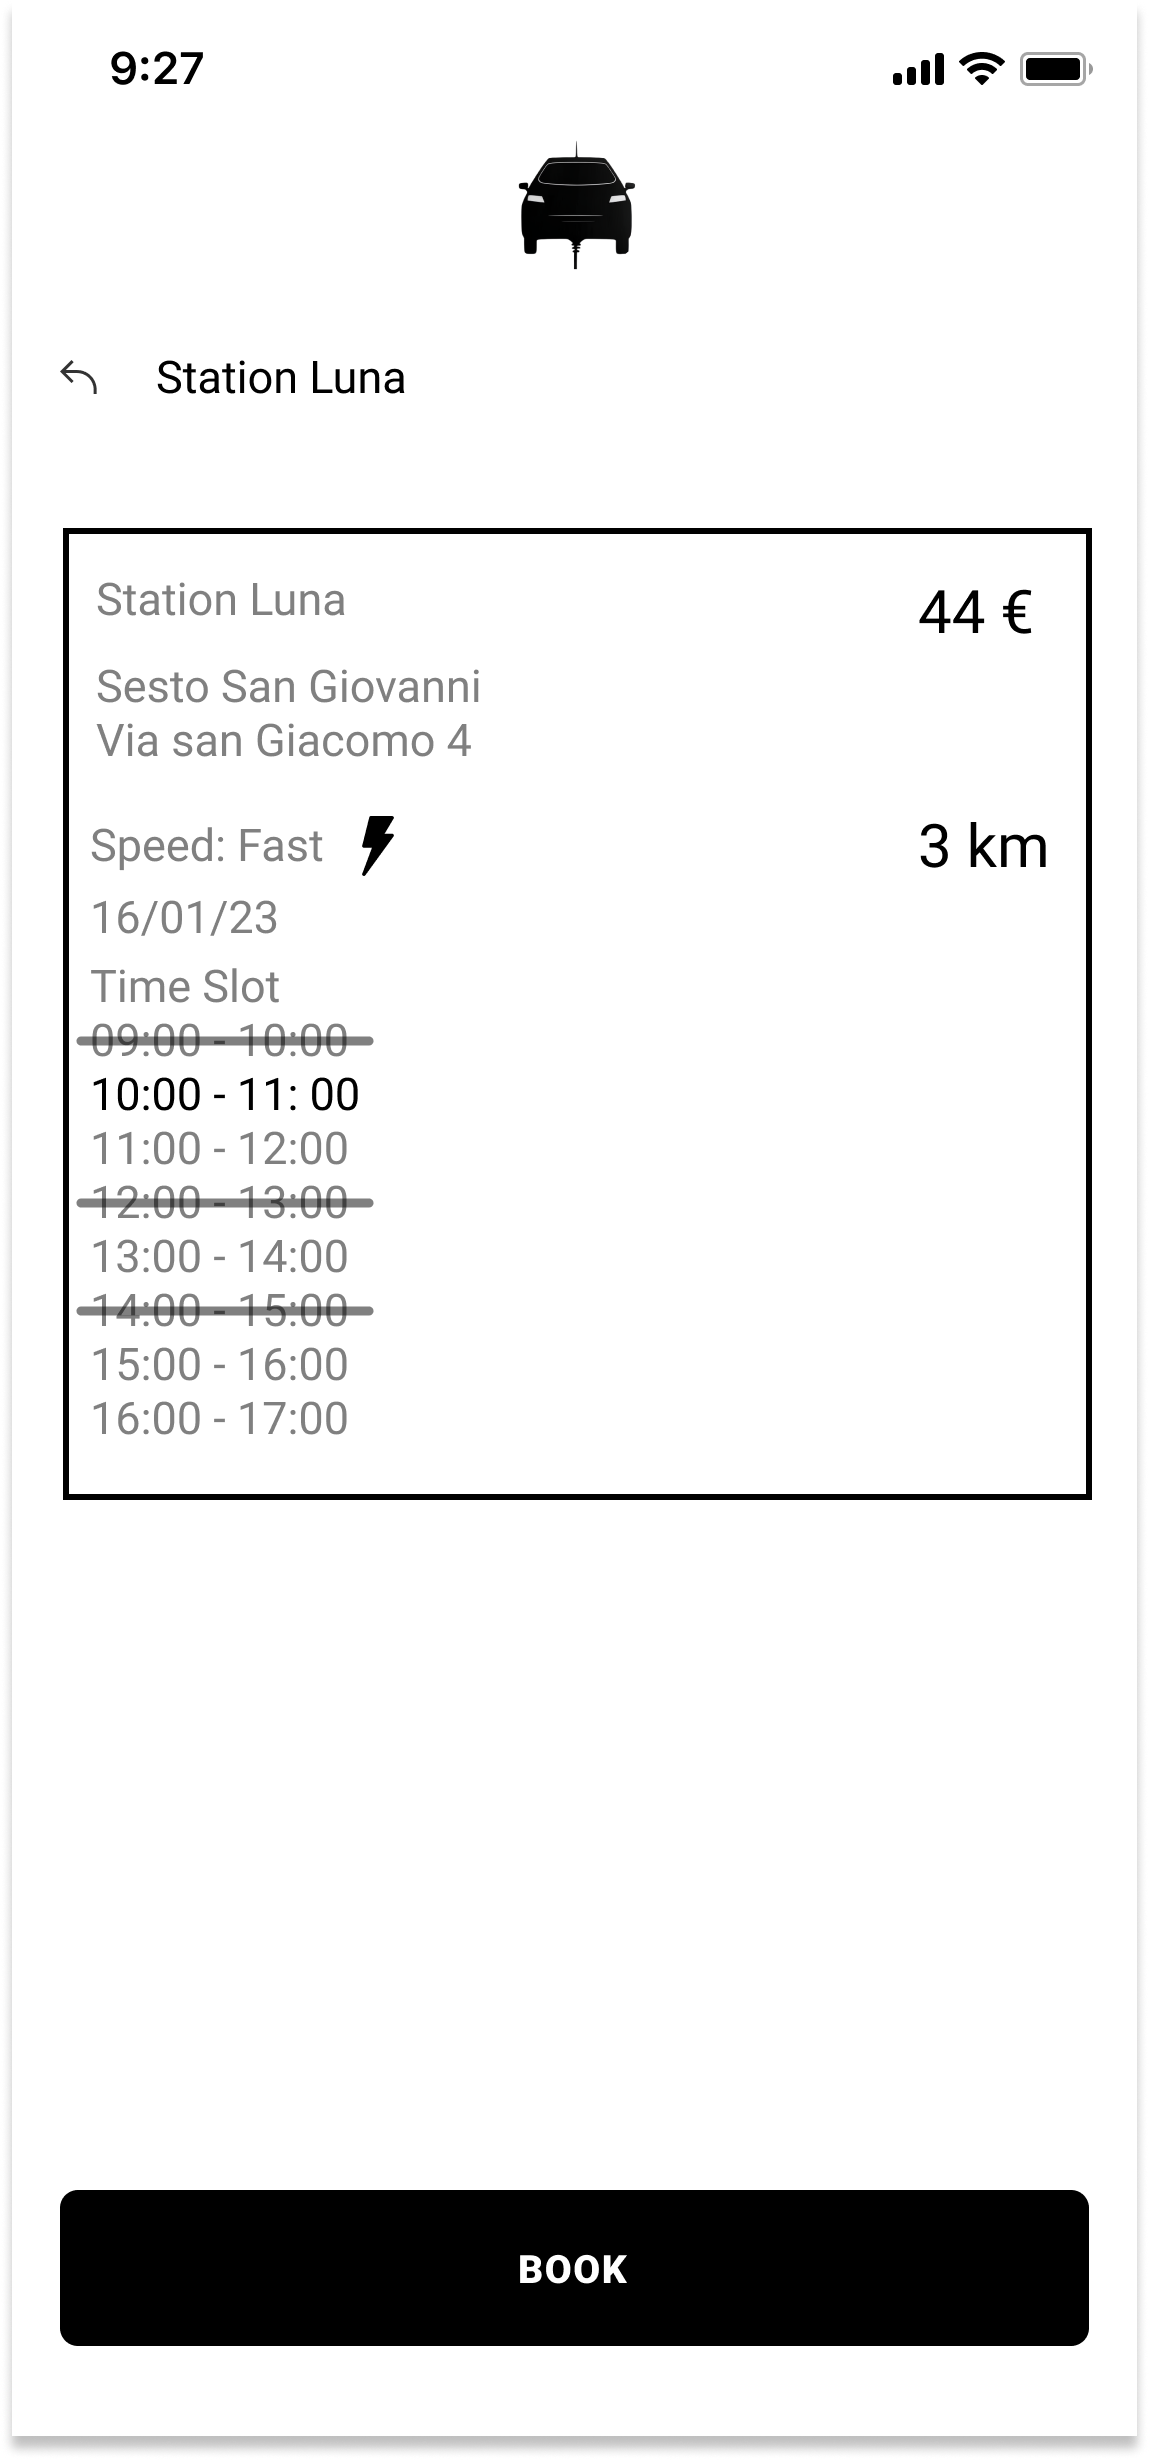
\includegraphics[keepaspectratio, height=15cm]{AppInterface/Station Details.png}
    \caption{User Checks Station Details}
    \label{fig:StationDetails}
\end{figure}
Here the user can book a charge, in the center of the screen the station details and a list of possible time frames are shown; the user can select the desired time frame by tapping on it. The selected time frame is bold while unavailable time frames are crossed. Once the user has selected the time frame he/her can proceed with the booking by clicking the book button opening \hyperref[pop:Booking]{the confirmation popup}. The user can return to the \hyperref[fig:Search]{search station page} by clicking the back arrow in the top left corner.
\begin{figure}[H]
    \centering
    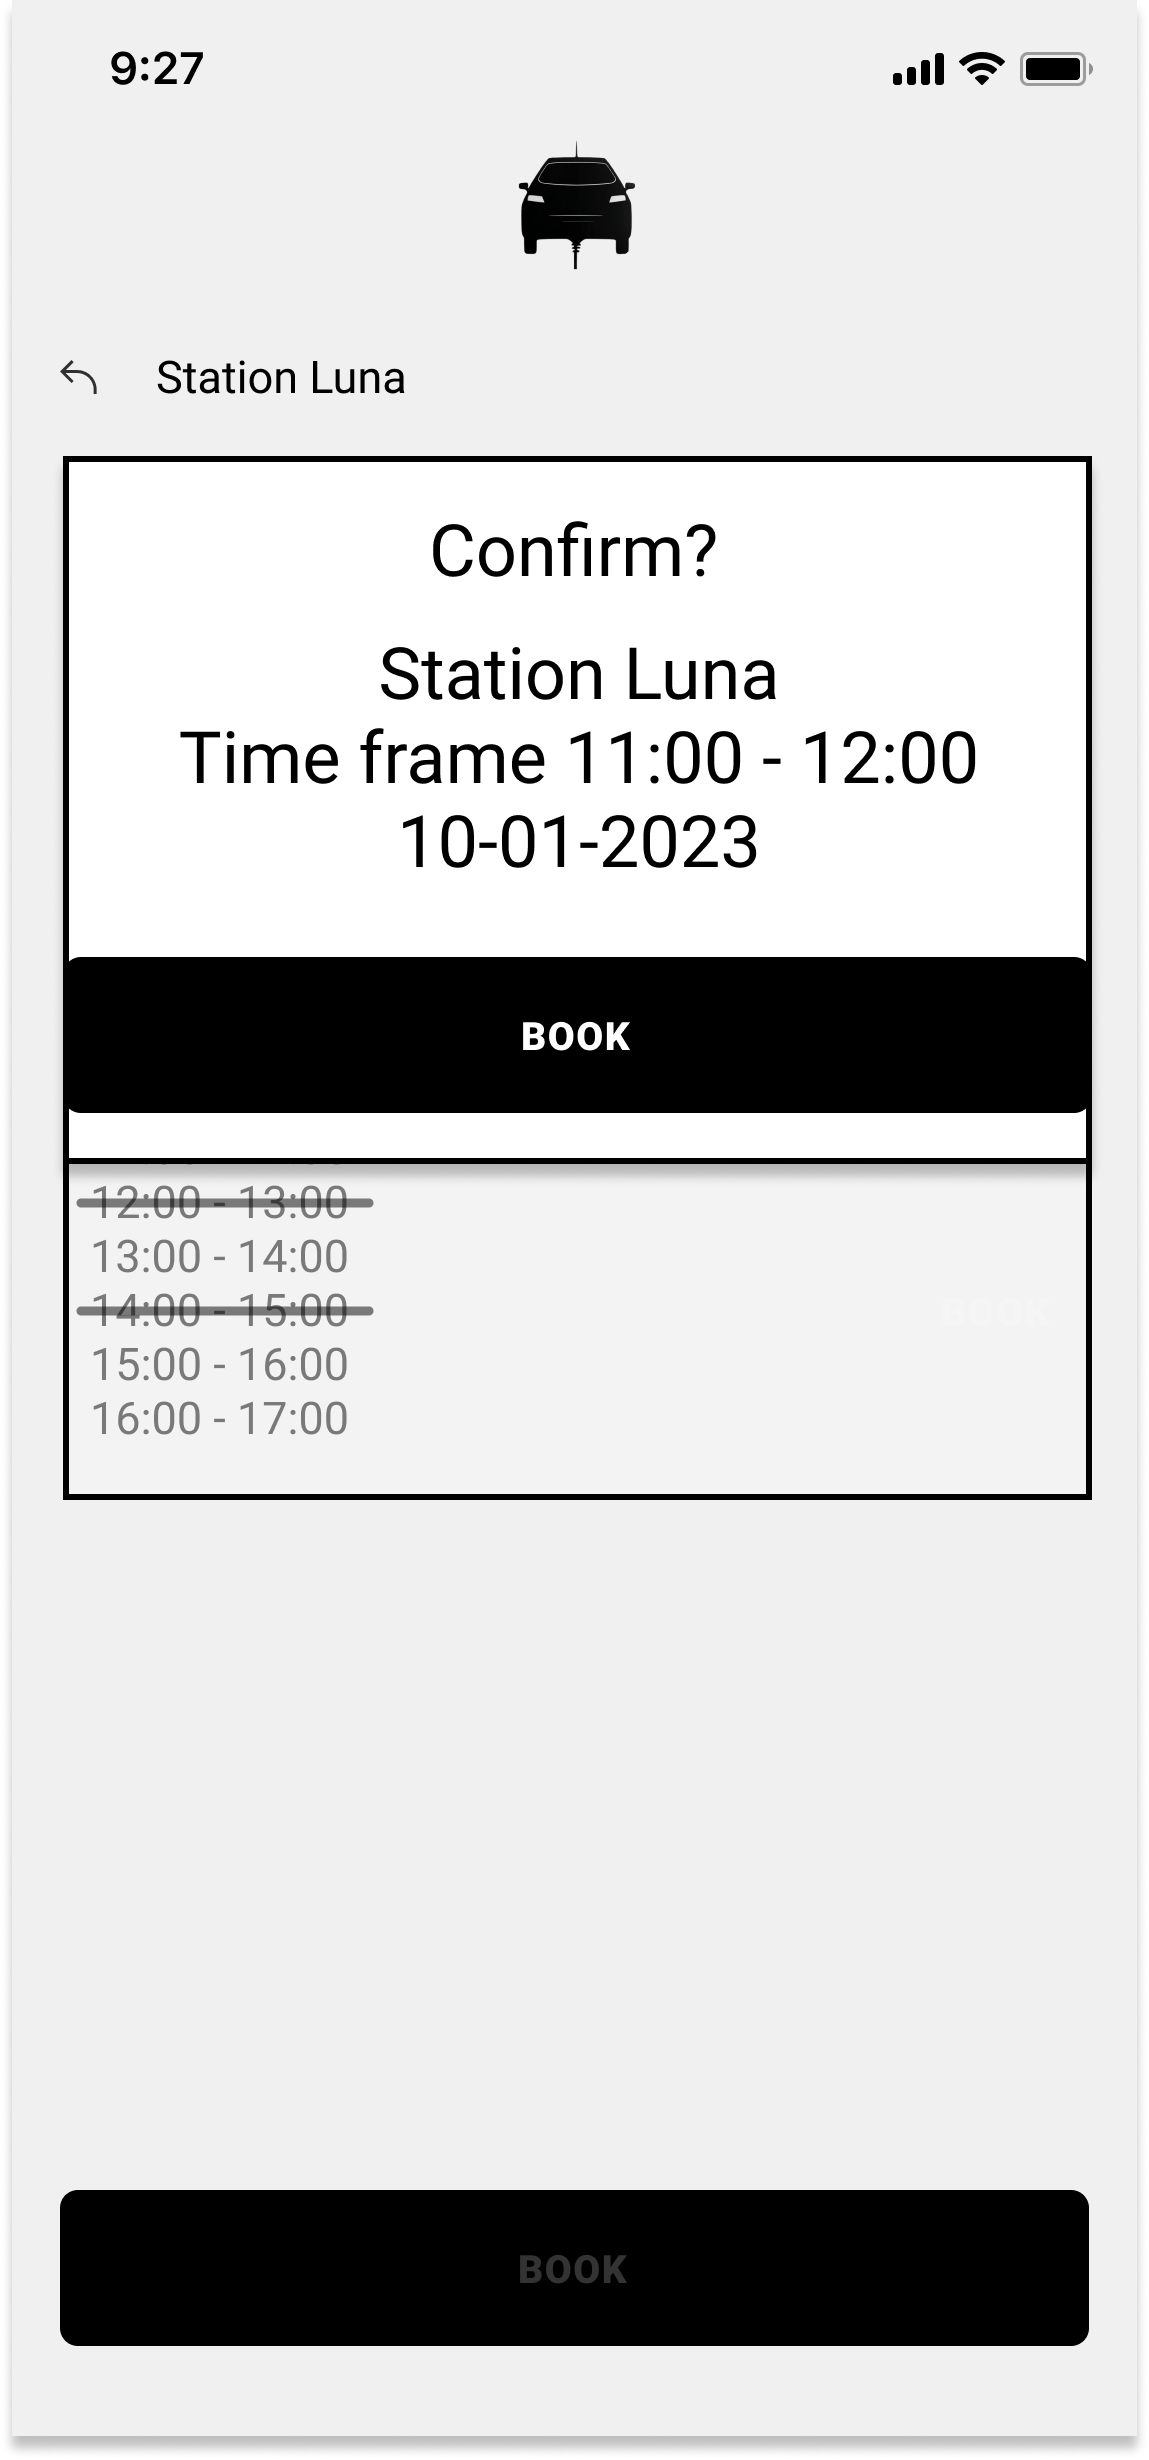
\includegraphics[keepaspectratio, height=15cm]{AppInterface/Book Confirmation.png}
    \caption{User Confirms the Booking}
    \label{pop:Booking}
\end{figure}
In this popup: station name, the selected date and time frame are displayed. The user can confirm the booking by pressing the Book button.
\subsubsection{Checks Booked Stations}
\begin{figure}[H]
    \centering
    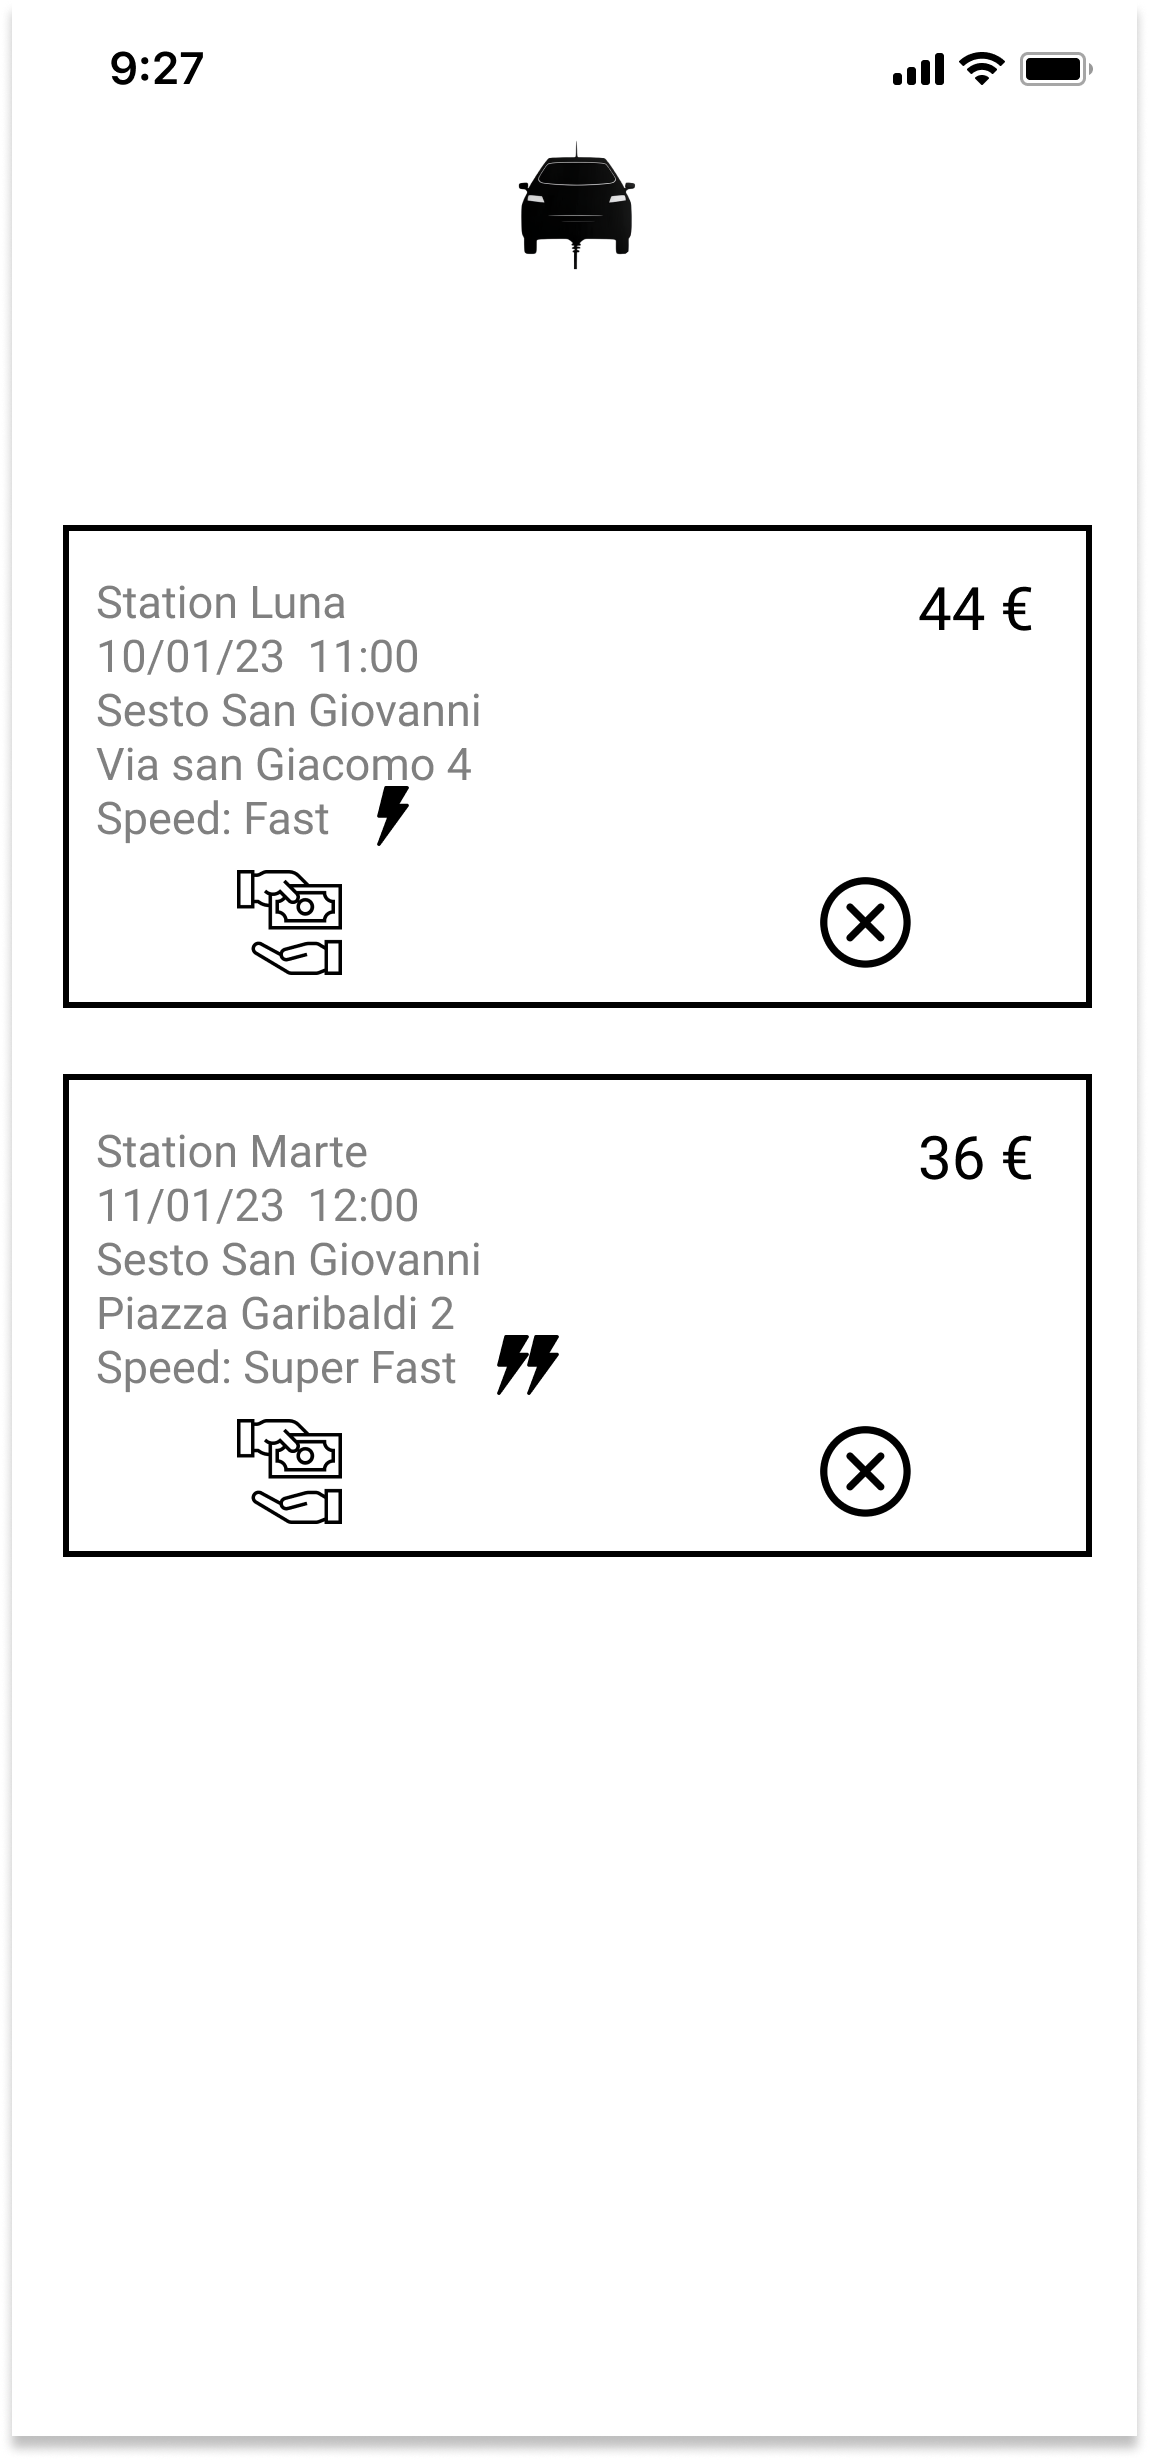
\includegraphics[keepaspectratio, height=15cm]{AppInterface/My Charges.png}
    \caption{User Manages Charges}
    \label{fig:myCharges}
\end{figure}
In this section the user can see a list his/hers booked charges; for each booking the name name, date, time frame and charge speed; the user can also pay for the charge by pressing the pay button and opening the \hyperref[pop:Pay]{pay popup} and delete a charge by pressing the delete button and opening the \hyperref[pop:Delete]{delete popup}.\\
By pressing the car logo the user can switch his/hers view to the \hyperref[fig:Search]{search page}.
\subsubsection{Pay a Charge}
\begin{figure}[H]
    \centering
    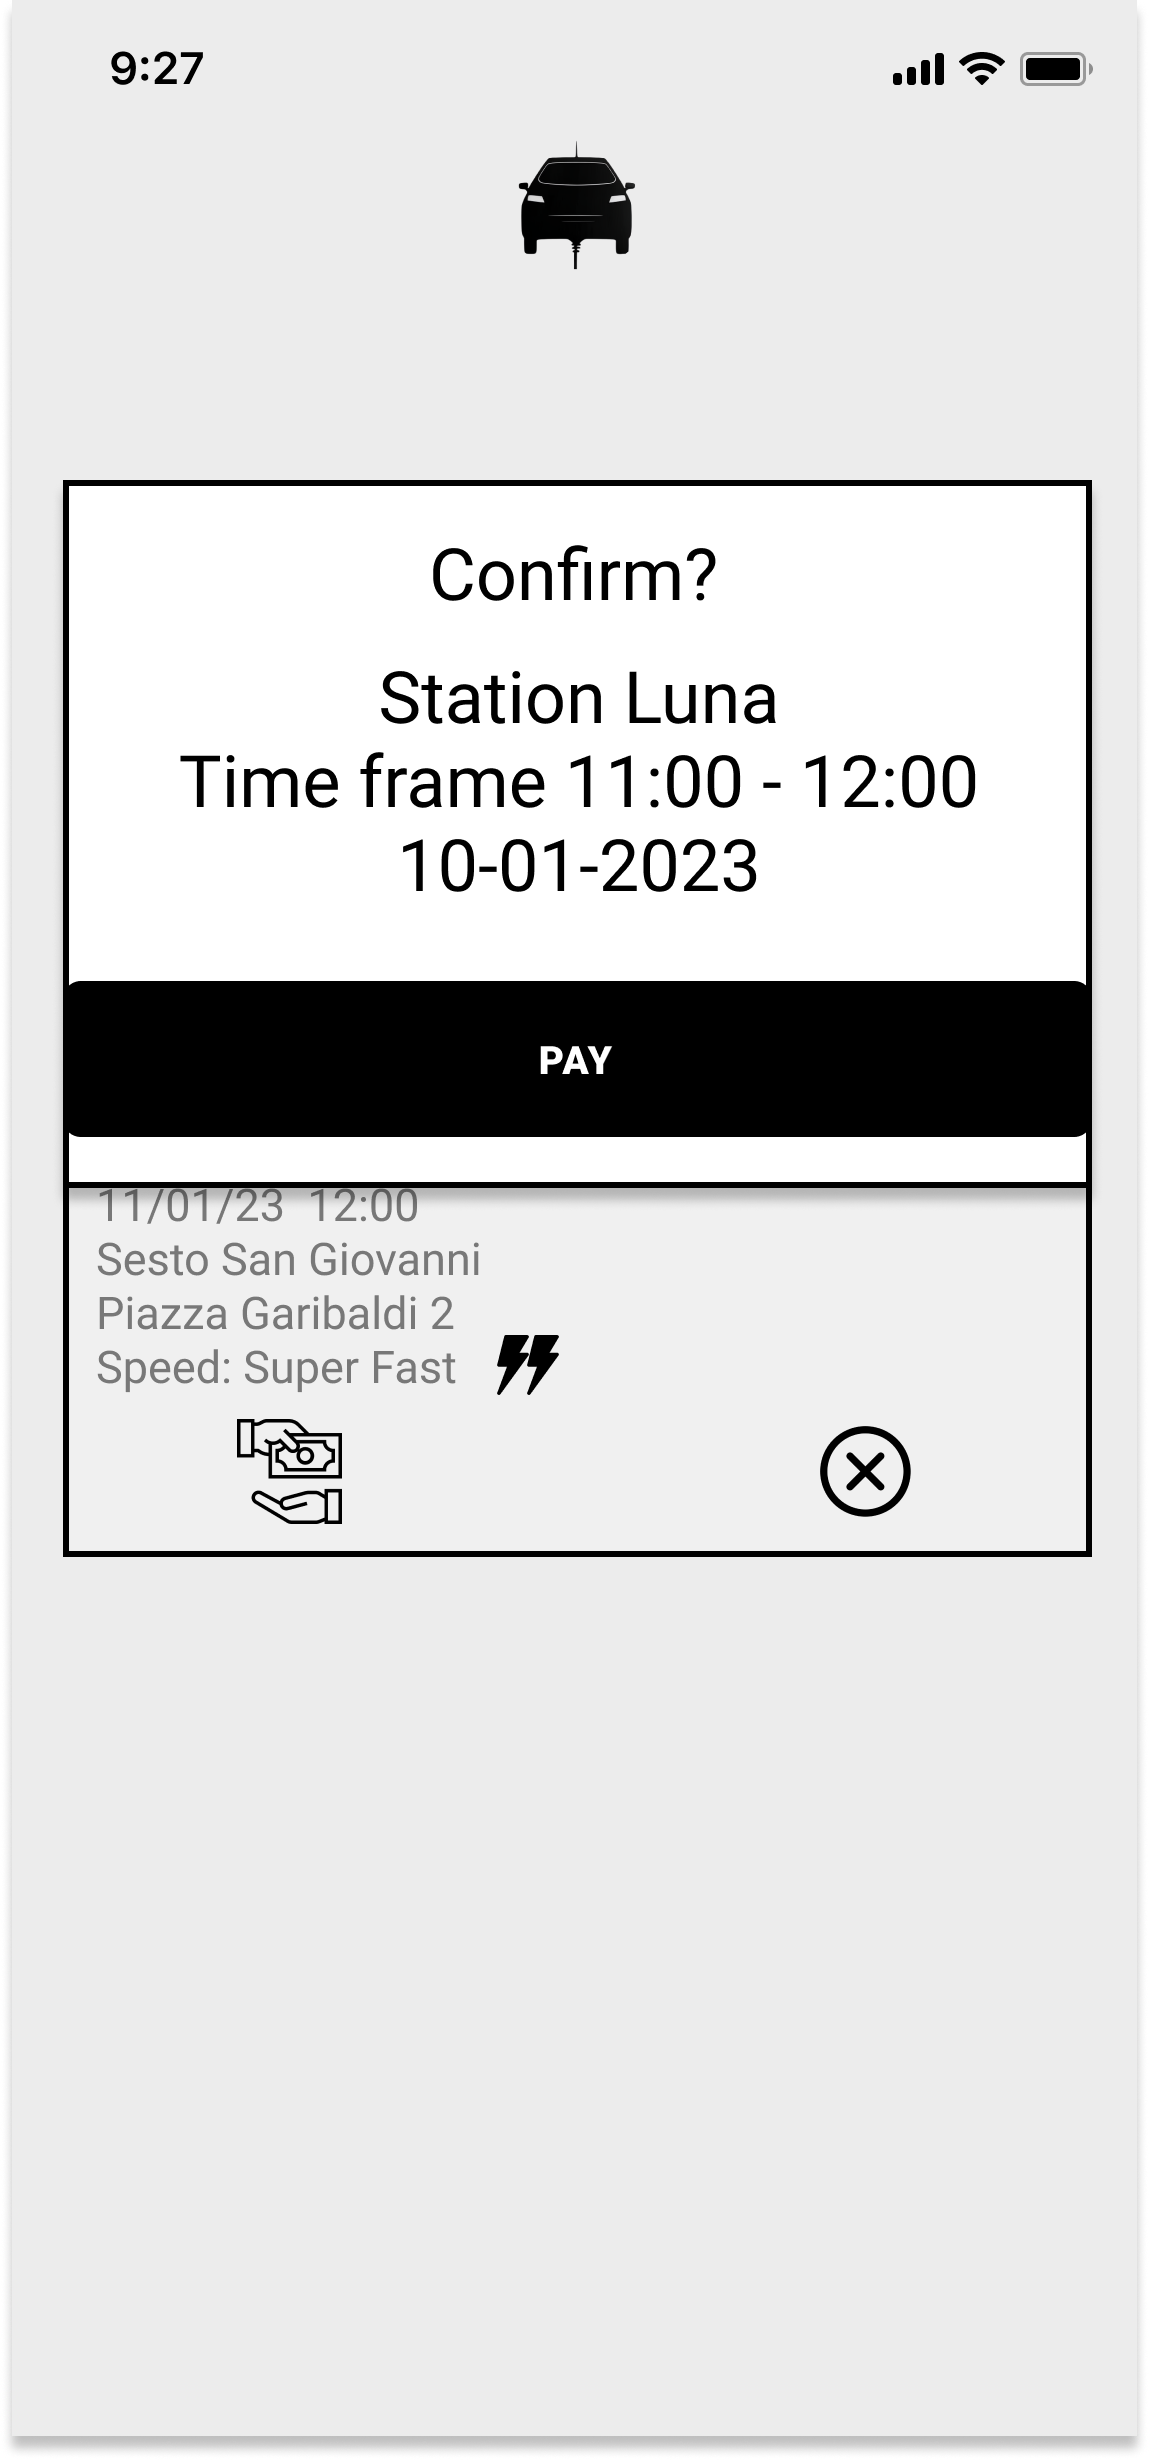
\includegraphics[keepaspectratio, height=15cm]{AppInterface/Pay Charge.png}
    \caption{User Pay a Charge}
    \label{pop:Pay}
\end{figure}
In this section the detail of the charge are displayed and the user can pay the charge by pressing the pay button.
\subsubsection{Cancel a Charge}
\begin{figure}[H]
    \centering
    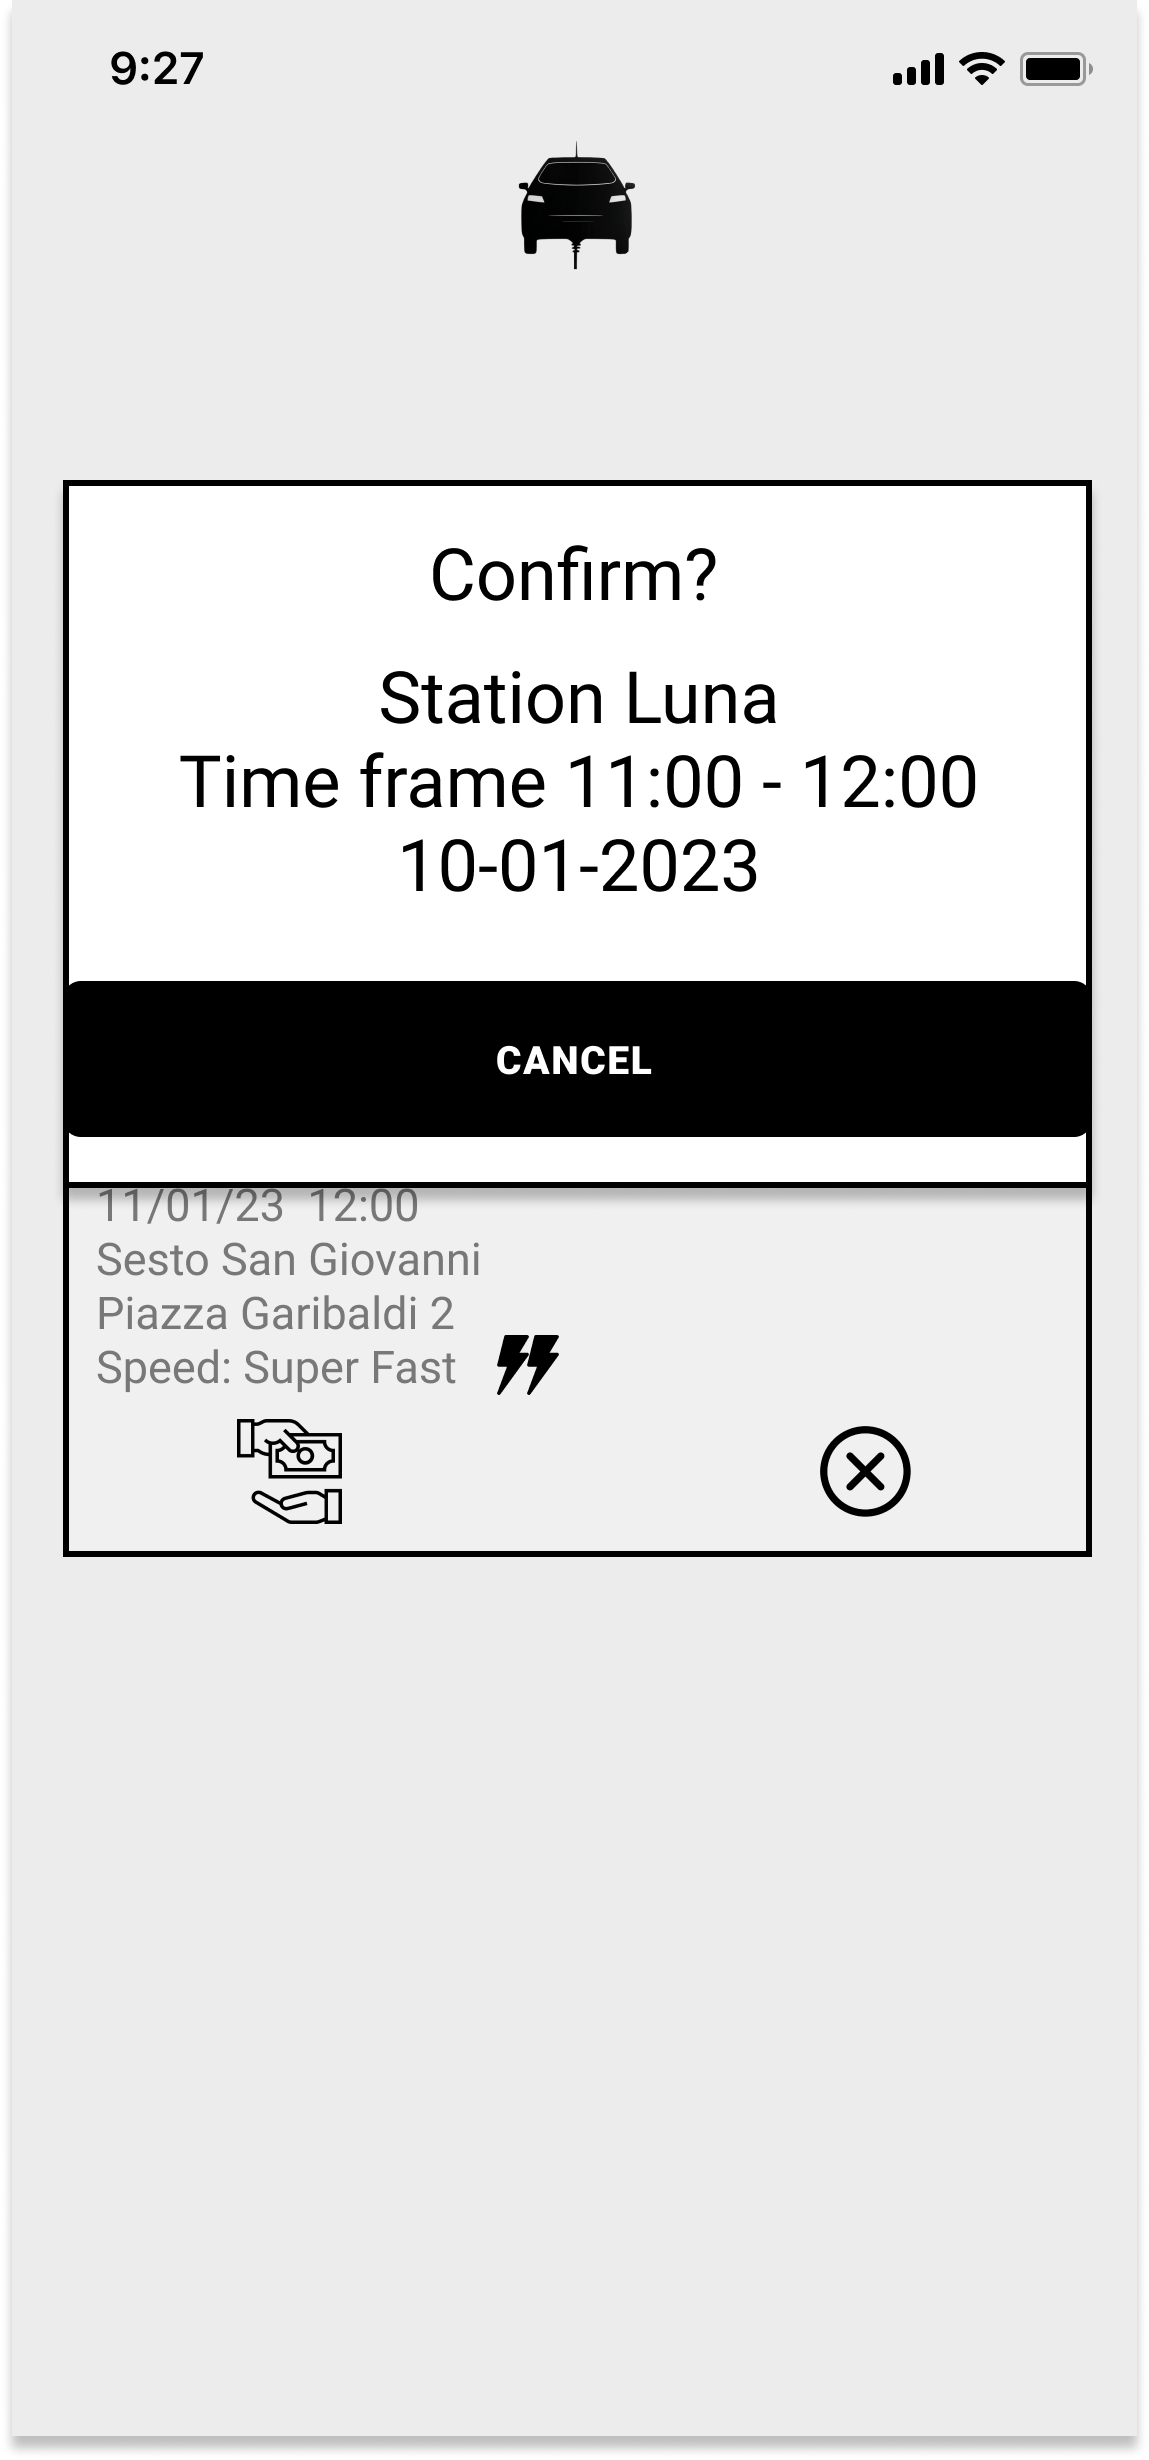
\includegraphics[keepaspectratio, height=15cm]{AppInterface/Delete Charge.png}
    \caption{User Cancel a Charge}
    \label{pop:Delete}
\end{figure}
In this section the detail of the charge are displayed and the user can cancel the charge by pressing the cancel button.
\subsection{CPO}
This section show the interface for the \ac{CPO}.
\subsubsection{Login}
\begin{figure}[H]
    \centering
    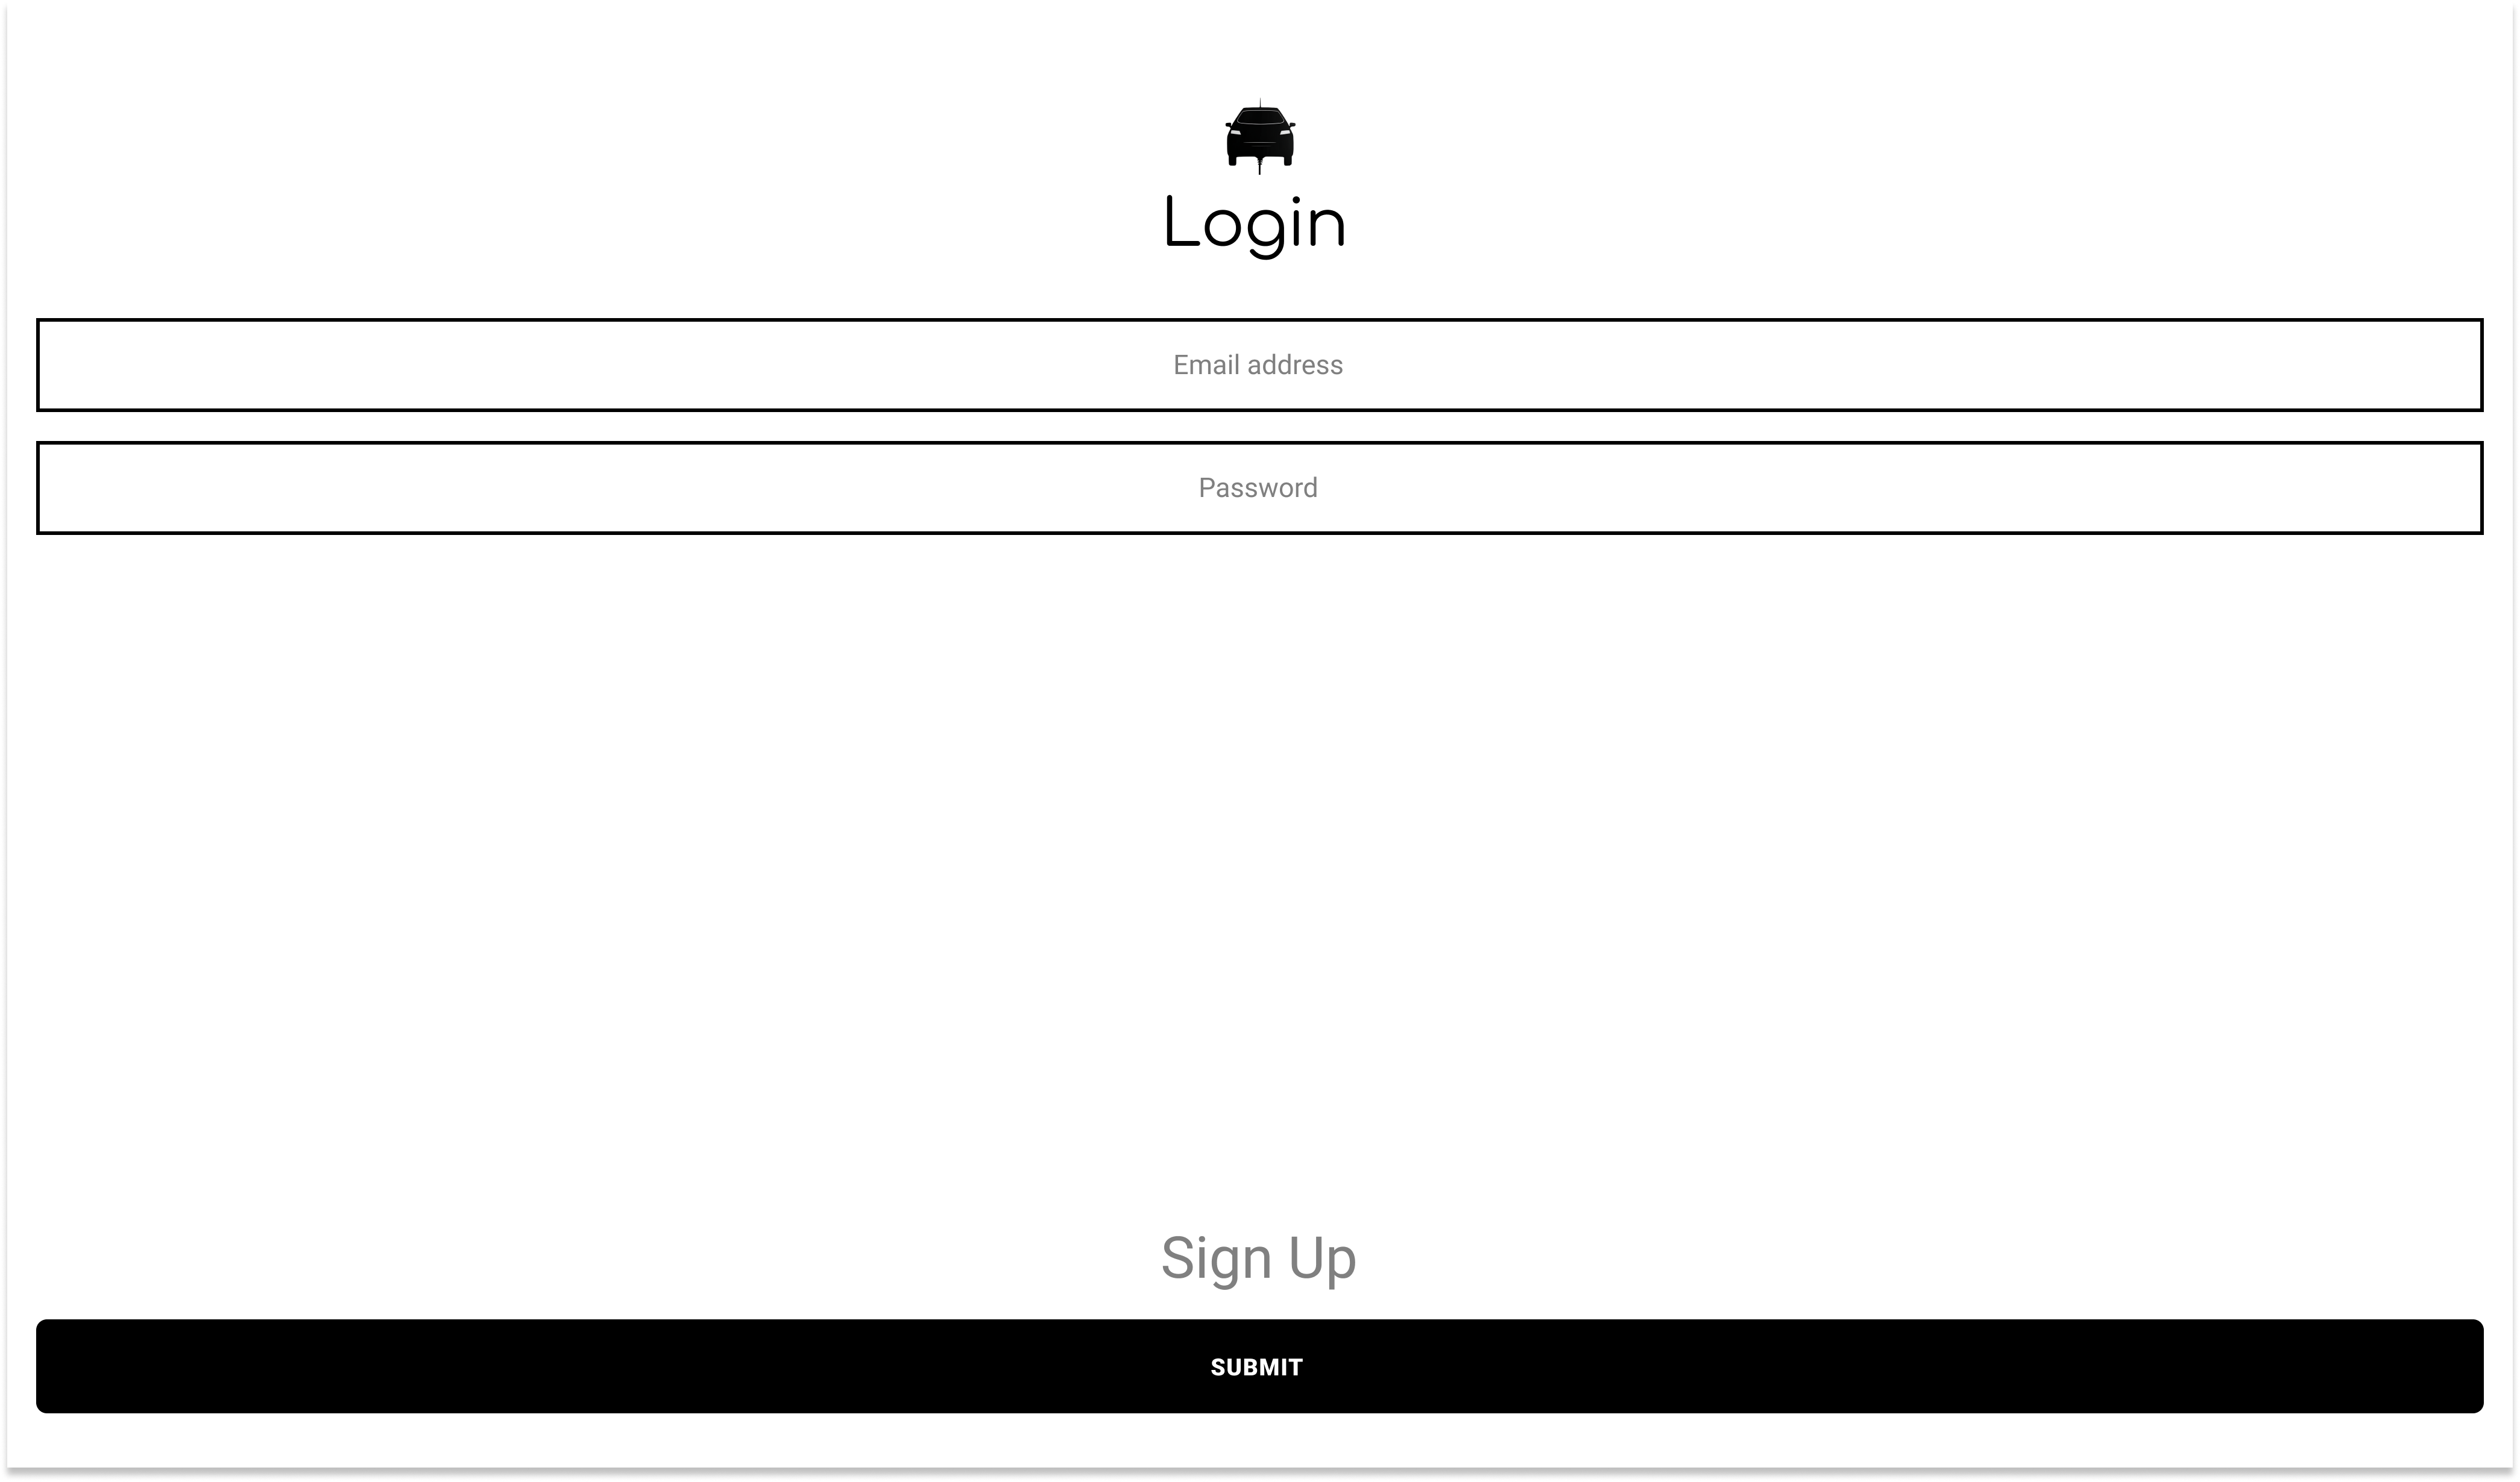
\includegraphics[keepaspectratio, width=15cm]{SiteInterface/Login.png}
    \caption{\ac{CPO} Login}
    \label{site:Login}
\end{figure}
Once the \ac{CPO} connects to the site this page is displayed. Here the \ac{CPO} can log into the system inserting the email and password provided during the registration. When the user press the submit button, if the information provided are correct, the \hyperref[site:Homepage]{homepage} is loaded.\\
If the \ac{CPO} is not registered it can by pressing the Sign Up button which loads the \hyperref[site:Register]{register page}.
\subsubsection{Register}
\begin{figure}[H]
    \centering
    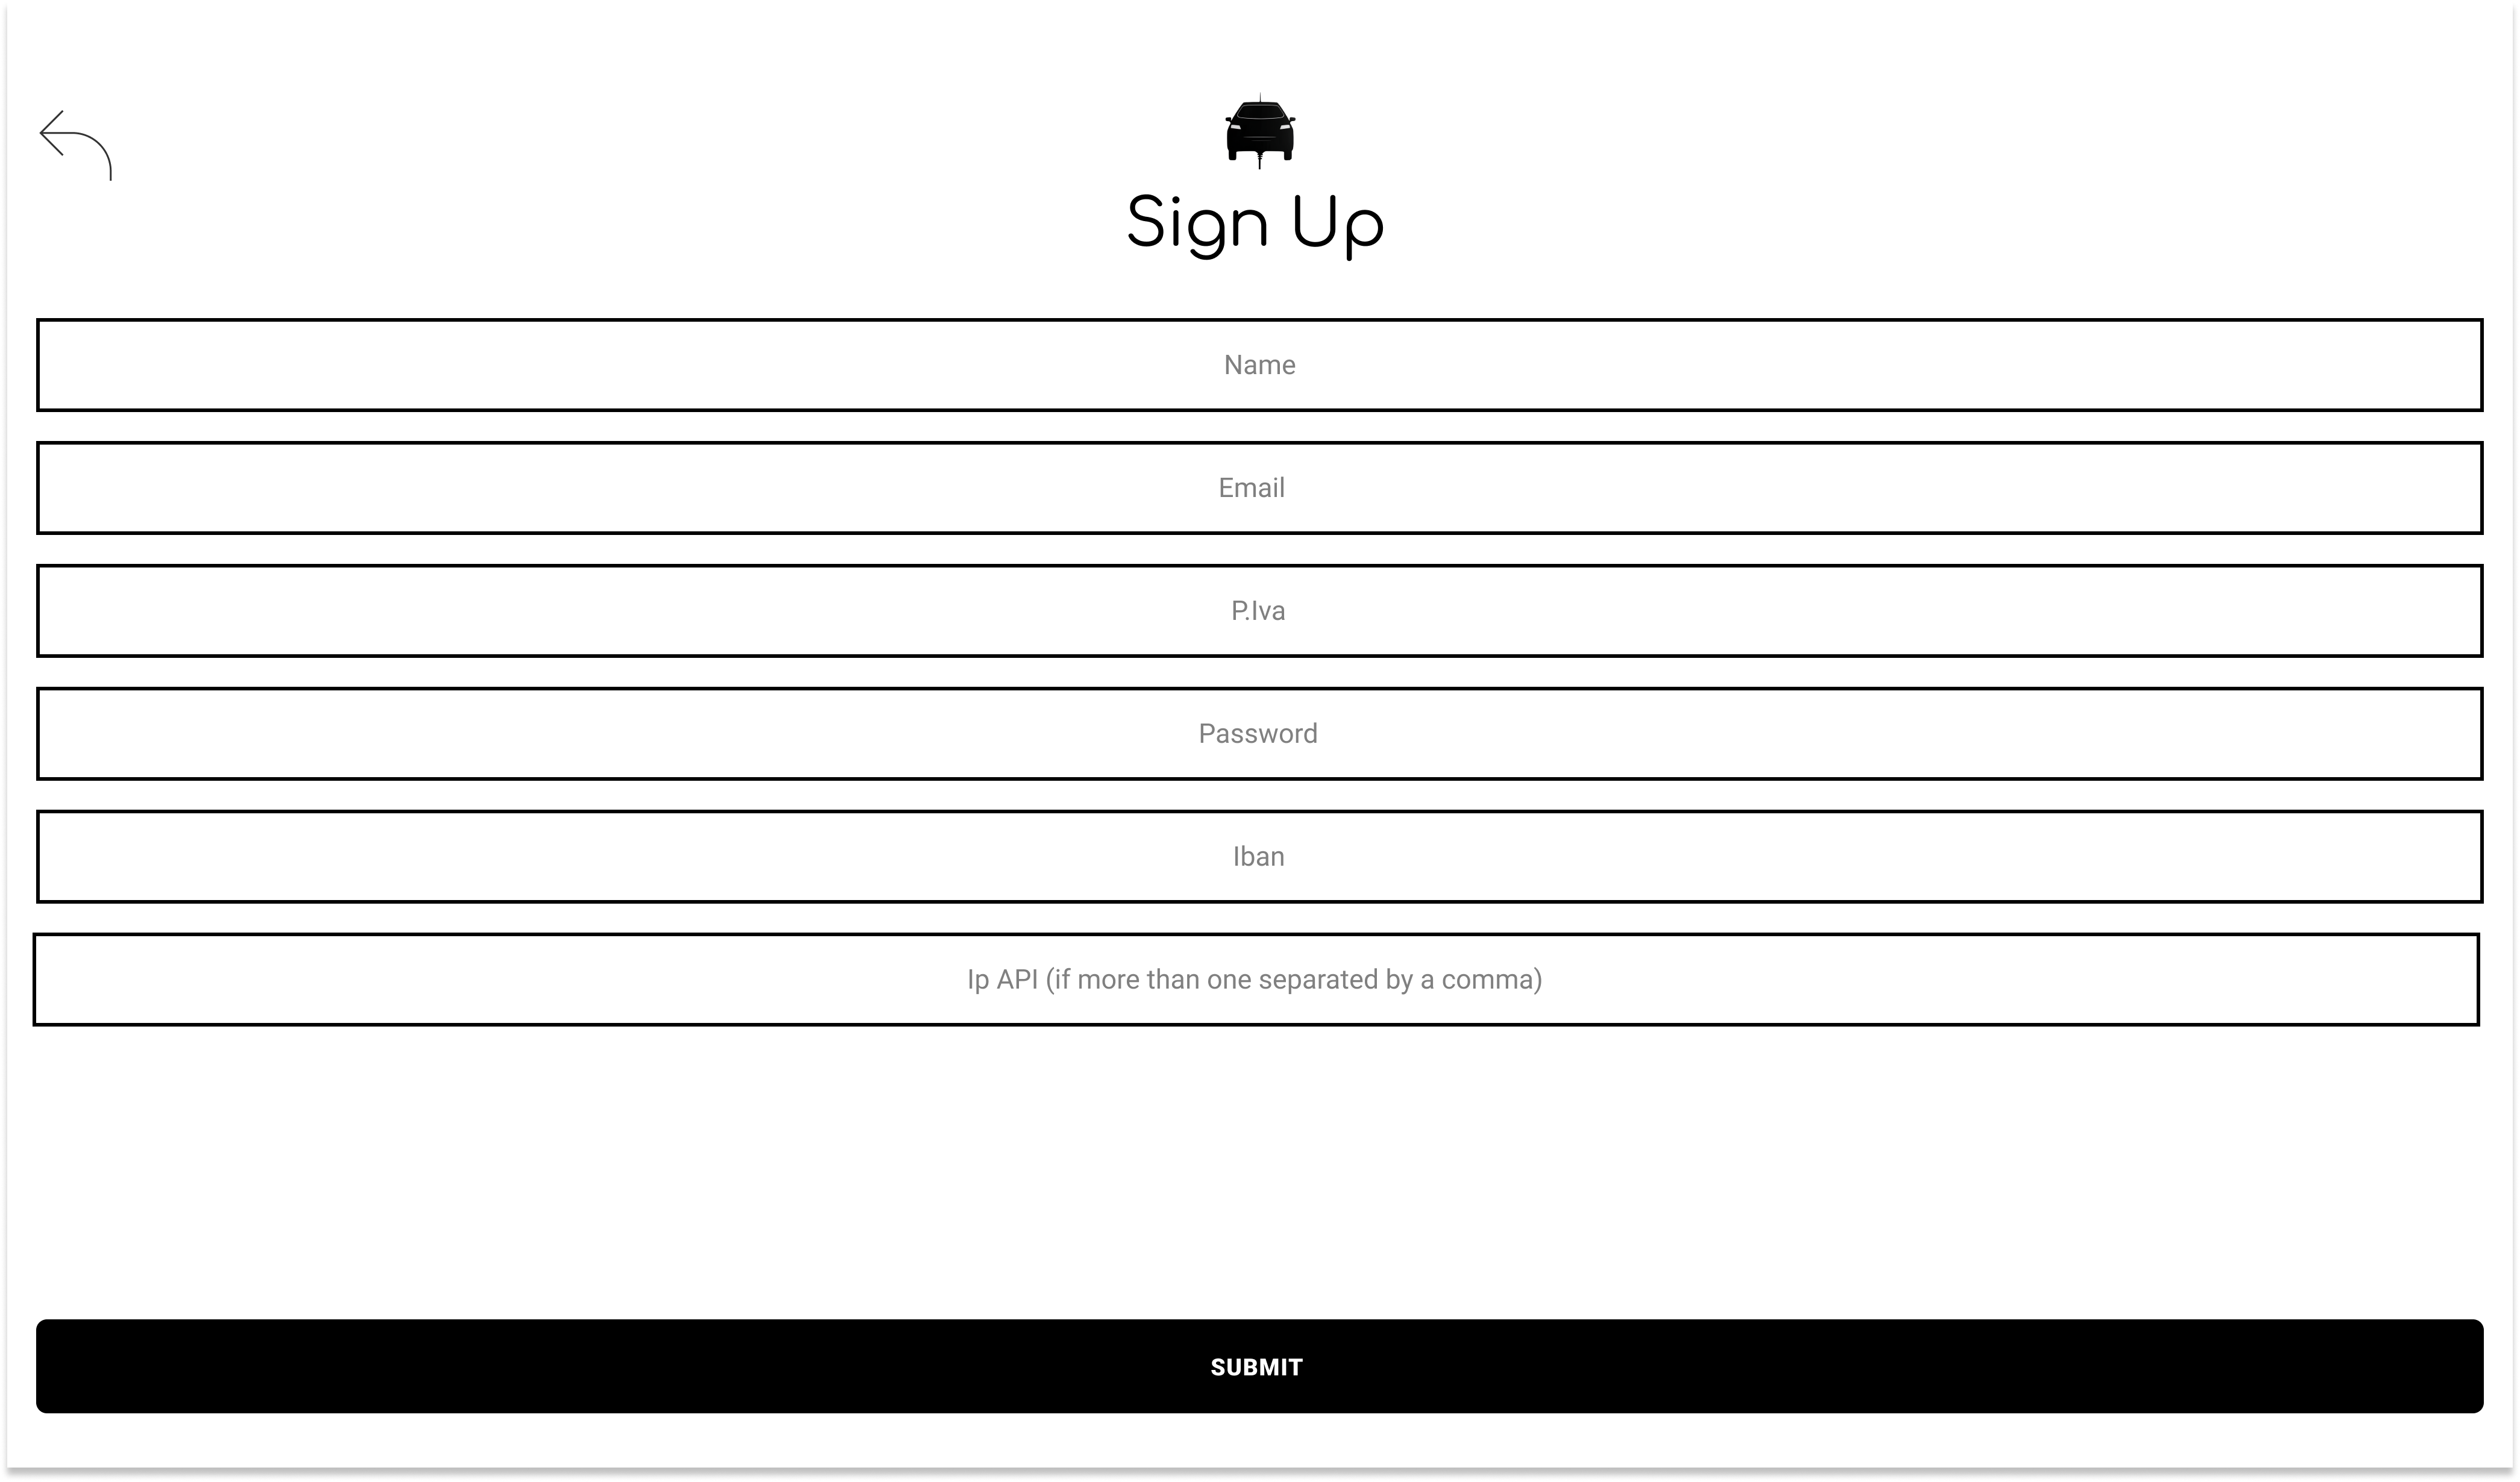
\includegraphics[keepaspectratio, width=15cm]{SiteInterface/Register.png}
    \caption{\ac{CPO} Register}
    \label{site:Register}
\end{figure}
In this page the \ac{CPO} can register itself to the service by providing the asked information, pressing the submit button and completing the registration; once the procedure is finished the \hyperref[site:Login]{login page} is displayed and the user is asked to log in the system.
\subsubsection{Home Page}
\begin{figure}[H]
    \centering
    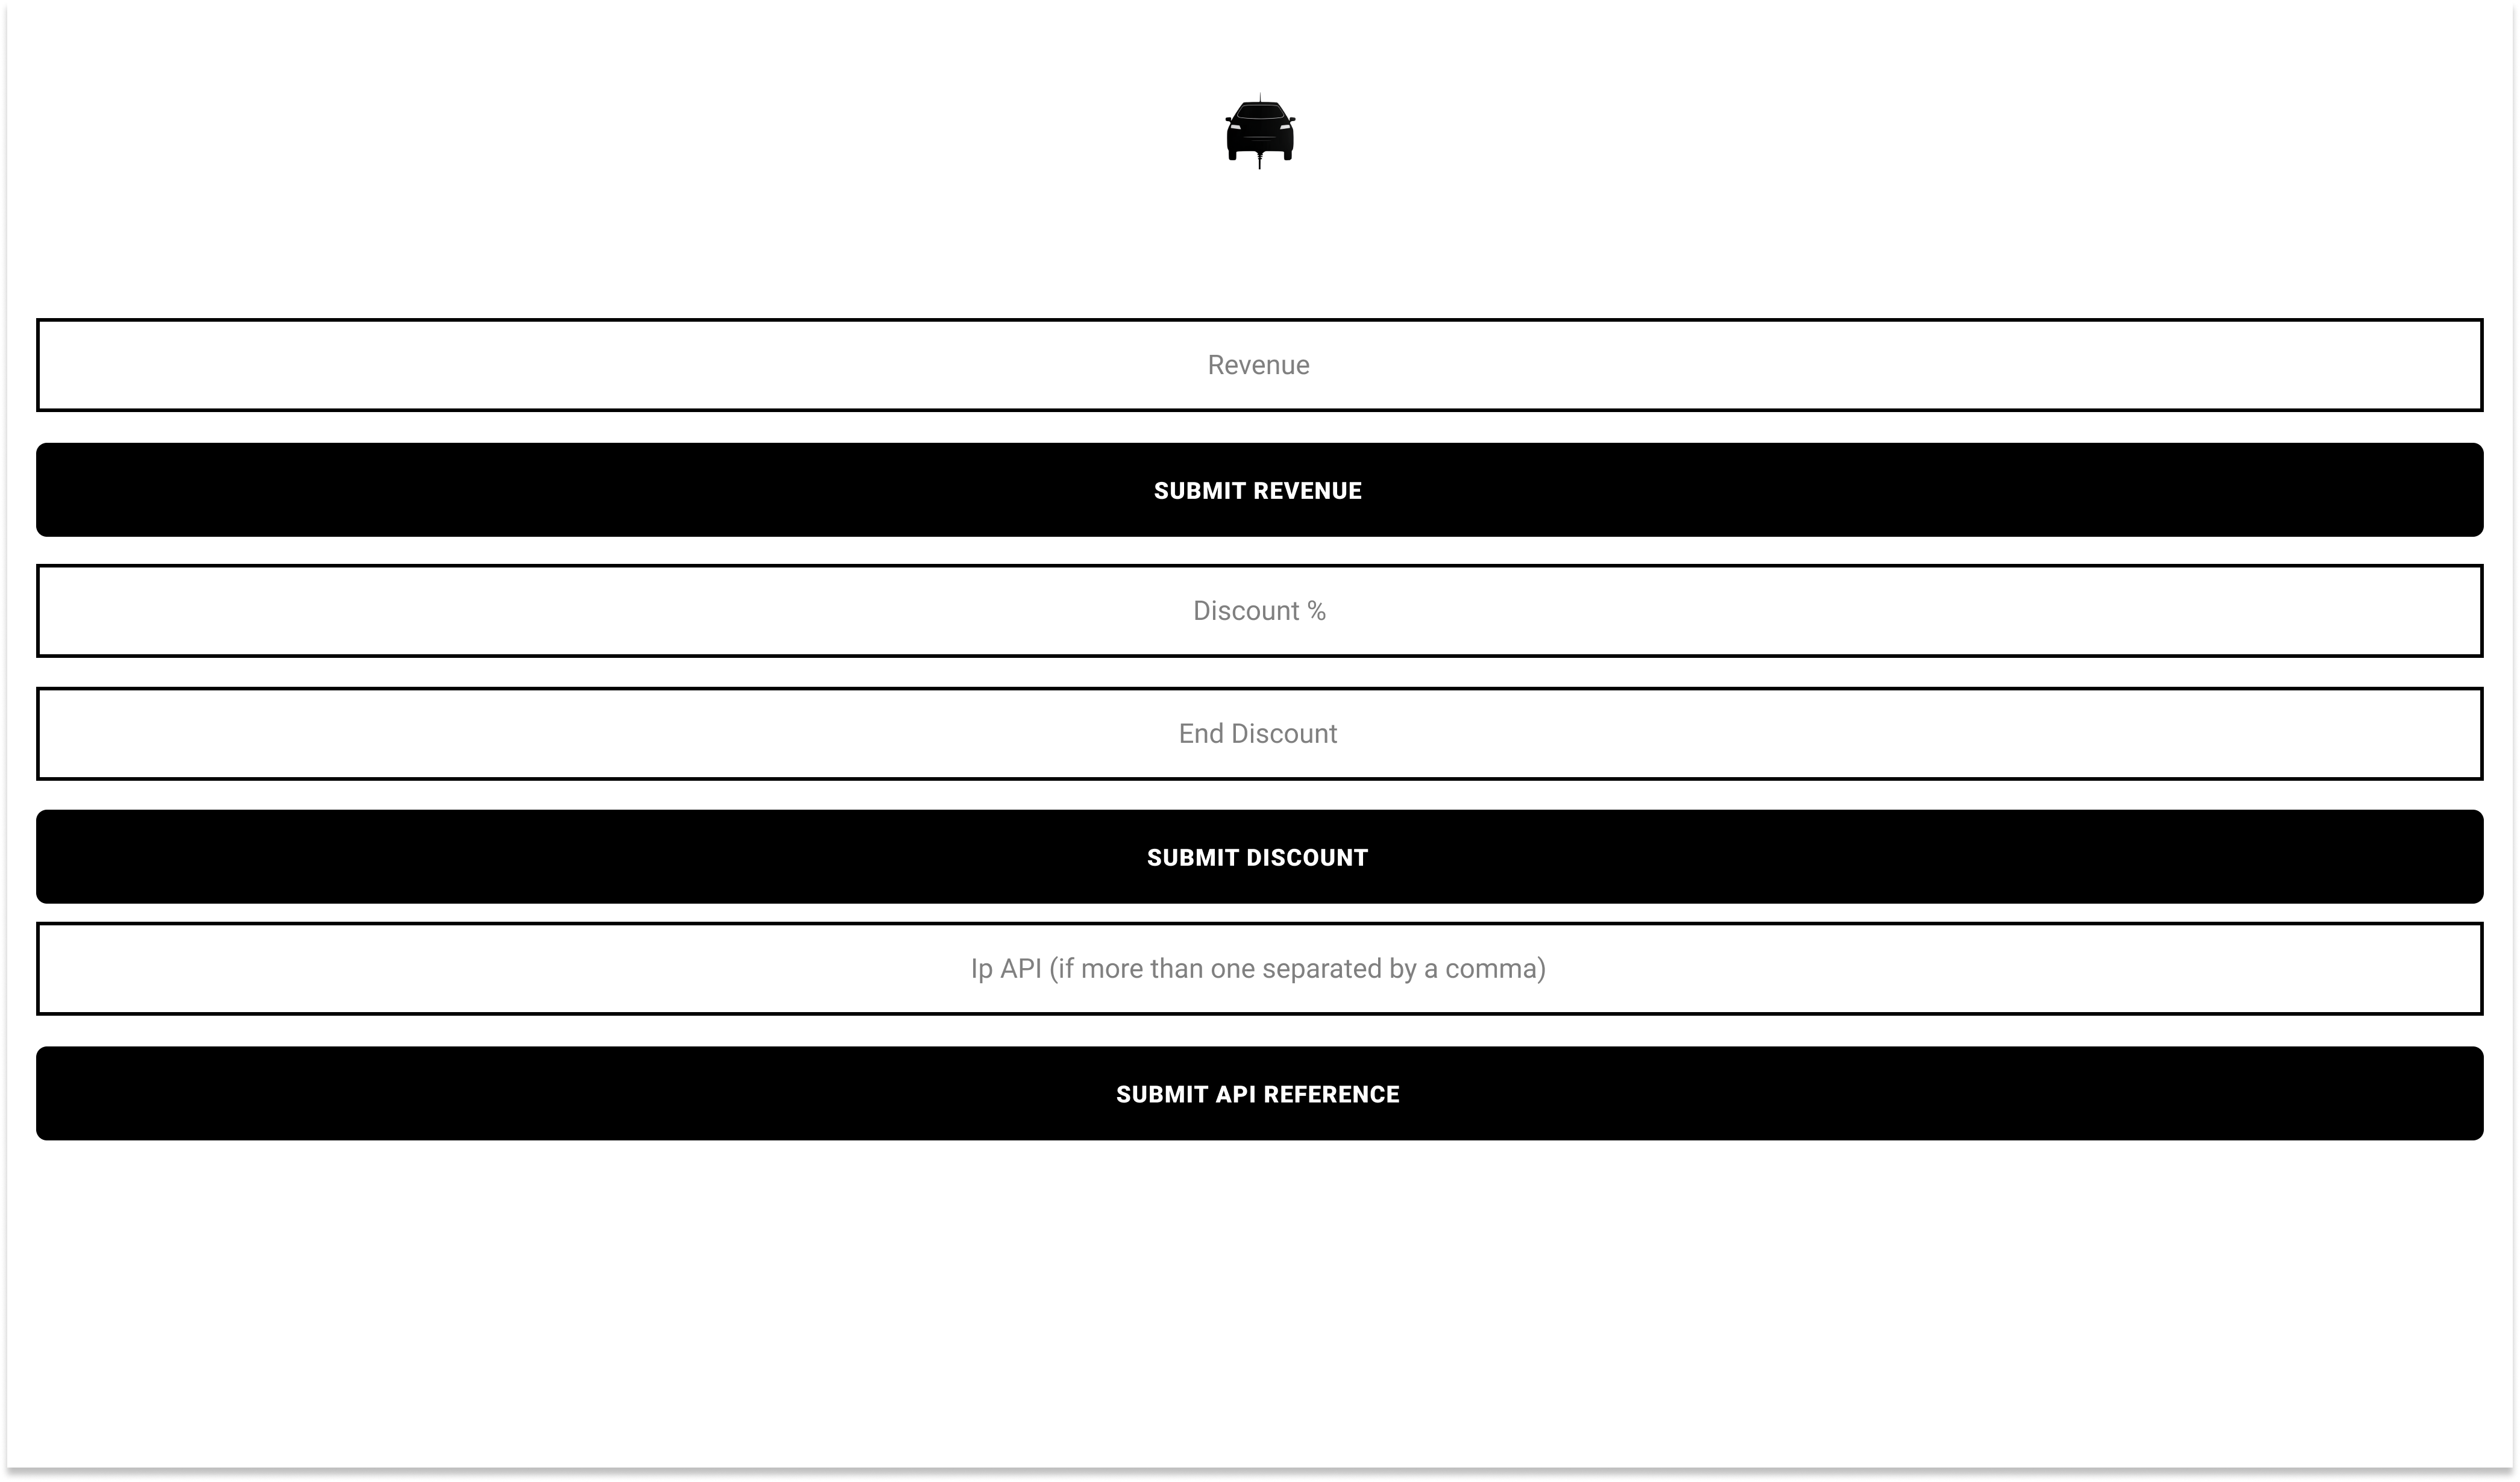
\includegraphics[keepaspectratio, width=15cm]{SiteInterface/Homepage.png}
    \caption{\ac{CPO} access the site functions}
    \label{site:Homepage}
\end{figure}
In this page the \ac{CPO} can change the revenue, create discounts and add cpms reference.\\
To change the Revenue the user has to insert the new revenue in the field and press the submit revenue button, the revenue will be updated and the page refreshed.\\
To create new discounts the user hast to insert the percentage of discounts, the end date of the discount and press the submit discount button, the discount will be updated and the page refreshed.\\
To add new Cpms the user has to insert the IP to the cpms ( if more than one separated by a comma) and press the submit api reference button, the api reference will be updated and the page refreshed.\\


\clearpage